% !TEX root =  ../MAIN.tex

\subsection{Approach}

\begin{figure}[tb]
	\centering
		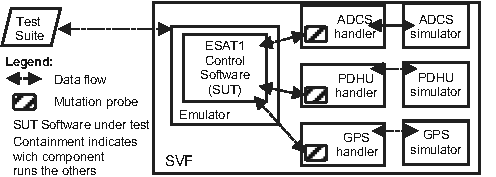
\includegraphics[width=8.4cm]{damat/images/dataMutationExample}
		\caption{\CHANGED{Data mutation probes integrated into \ESAIL.}}
		\label{fig:appr:mutateProbesInserted}
	\end{figure}

\begin{figure}[tb]
	\centering
		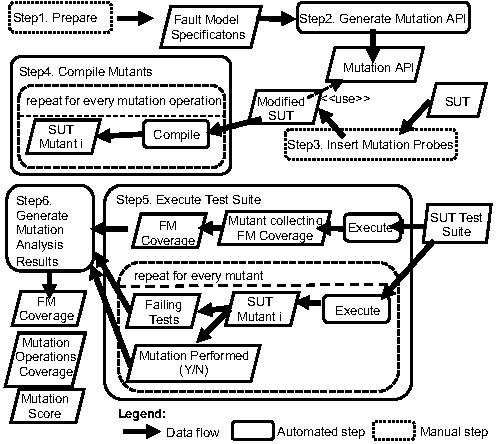
\includegraphics[width=8cm]{damat/images/dataDrivenBufferProcess}
		\caption{The \APPR process.}
		\label{fig:appr:approach}
	\end{figure}

\subsubsection{Overview}


\INDEX{Data-driven mutation analysis} aims to evaluate the effectiveness of a test suite in detecting \INDEX{semantic interoperability \UPDATED{faults}}. 
It is achieved by modifying (i.e., mutating) the data exchanged by CPS components. It generates \INDEX{mutated data} that is representative of data that might be observed at runtime in the presence of a component that behaves differently than expected in the test case; also, it mutates  data that is not automatically corrected by the software 
(e.g., through cyclic redundancy check codes)
%(e.g., through CRC mechanisms, which aim to correct technical interoperability problems) 
and thus causes software failures (i.e., the mutated data shall have a different semantic than the original data). For these reasons, data mutation is driven by a fault model specified by the engineers based on domain knowledge.

Although different types of fault models might be envisioned,
%see background
in this paper we propose a technique (\INDEX{data-driven mutation analysis with tables}, \APPR),
which automates data-driven mutation analysis by relying on
a tabular \CHANGED{block model}, itself tailored to the \UPDATED{SUT} through predefined mutation operators.
To concretely perform data mutation at runtime, \APPR relies on a set of \INDEX{mutation probes} that shall be integrated by software engineers into the software layer that handles the communication between components. The runtime behaviour of mutation probes (i.e, what data shall be mutated and how) is driven by the fault model. Thus, \APPR can automatically generate the implementation of mutation probes from the provided fault model.
Depending on the CPS, probes might be inserted either into the \UPDATED{SUT}, into the simulator infrastructure, or both.
Figure~\ref{fig:appr:mutateProbesInserted} shows the architecture of the \ESAIL satellite system (one of the subjects considered in our empirical evaluation) with mutation probes integrated into the SVF\footnote{Software Validation Facility~\cite{Isasi2019}; it usually includes one or more simulators, an emulator to run the code compiled for the target hardware, and test harnesses.} functions that handle communication with external components (PDHU, GPS, and ADCS in this case). 



\APPR works in six steps, which are shown in Figure~\ref{fig:appr:approach}. 
In Step 1, based on the provided methodology and predefined mutation operators, the engineer prepares a fault model specification tailored to the SUT.
% capturing the data format and the types of faults that shall be injected for every data item exchanged by the system components.
In Step 2, \APPR generates a mutation API with the functions that modify the data according to the provided fault model.
In Step 3, the engineer modifies the \UPDATED{SUT} by introducing mutation probes (i.e., invocations to the mutation API) into it.
\REVTOOL{P-2}{Instead of modifying the SUT the engineer may modify the test harness (e.g., the SVF simulator); such choice depends on the software under test, if the test cases are executed through a simulator, such choice prevents introducing damaging changes into the SUT (e.g., delay task execution and break strict real-time requirements).}
In Step 4, \APPR generates and compiles mutants. 
Since the \APPR mutation operators may generate mutated data by applying multiple mutation procedures, \APPR may generate several mutants, one for each \UPDATED{mutation operation (i.e., a mutation procedure configured for a data item, according to our terminology, see Section~\ref{sec:mutantsGeneration})}.
In Step 5, \APPR executes the test suite with all the mutants including a mutant (i.e., the coverage mutant) which does not  modify the data but traces the coverage of the fault model.
In Step 6, \APPR generates mutation analysis results.

%\UPDATED{
%In our context, the \emph{software under test (SUT)} is the CPS embedded software that is verified by a test suite, which is the target of data-driven mutation analysis. Therefore, we refer to the software developed by the engineers as the \emph{original SUT}. An \emph{SUT mutant} (simply, a \emph{mutant}) is a version of the SUT that integrates a \emph{mutation probe} and shall make test cases fail. 
%%A mutation operator simulates one specific interoperability error (a specific type of that automatically alters data by applying one specific \emph{mutation operation}.
%}

In the following sections we describe the structure of our fault model and each step of \APPR.



\subsubsection{Fault Model Structure}
\label{sec:faultModelStructure}





The \APPR fault model enables the specification of the format of the data exchanged between components along with the type of faults that may affect such data. 
In this paper, we refer to the data exchanged by two components as \INDEX{message}; also, each CPS component may generate or receive different \INDEX{message types}.
For a single CPS, more than one fault model can be specified. For example, in the case of \ESAIL{} we have defined one fault model for every message type that could be exchanged by the three components under test (i.e., ADCS, PDHU, and GPS). In total, for \ESAIL, we have 14 fault models, 10 for the communication concerning ADCS (we have 10 different message types), 3 for PDHU, and 1 for GPS.

The \APPR fault model enables the modelling of data that is exchanged through a specific data structure: the data buffer. This was decided because it is a simple and widely adopted data structure for data exchanges between components in CPS. Also, more complex data structures (e.g., hierarchical ones like trees) are often flattened into data buffers in order to be exchanged by different components (e.g., through the network). When the CPS software is implemented in C or C++ (common CPS development languages) data buffers are implemented as arrays. Figure~\ref{fig:appr:bufferStructure} shows three block diagrams representing (part of) the buffer structure used to exchange messages of type InterfaceHouseKeeping and InterfaceStatus in \ESAIL.

A data buffer is characterized by a \INDEX{unit size} that specifies the dimension, in bytes, of the single cell of the underlying array and a \INDEX{buffer size}, which specifies the total number of units belonging to the buffer. Each data buffer can contain one or more \INDEX{data items}; the size of data items may vary as they may span over multiple units. Also, each data item is interpreted by the CPS software according to a specific \INDEX{representation} (e.g., integer, double, etc.). 
In \ESAIL, the unit size is one byte and the data items may span over one or two buffer units (see Figure~\ref{fig:appr:bufferStructure}). 
%Figure~\ref{} provides an example buffer instance for a \emph{Magnetorquer Set PWM RSP message}.

The \APPR fault model enables engineers to specify (1) the \emph{position} of each data item in the buffer, (2) their \emph{span}, and (3) their \emph{representation type}. Our current implementation supports six data representation types: int, long int, float, double, bin (i.e., data that should be treated in its binary form), hex (i.e., data that should be treated as hexadecimal).
Further, for each data item, \APPR enables engineers to specify one or more data faults using the mutation operator identifiers. For each operator, the engineer 
shall provide values for the required configuration parameters.

Table~\ref{table:operators} provides the list of mutation operators included in \APPR along with their description. The \APPR mutation operators generate \INDEX{mutated data item instances} through one or more \INDEX{mutation procedures}, which are the functions that generate a mutated data item instance given a correct data item instance observed at runtime. For example, the \emph{VAT} operator includes only one mutation procedure (i.e., setting the current value above the threshold) while the \emph{VOR} operator includes two mutation procedures, which are
(1) replacing the current value with a value above the specified valid range and (2) replacing the current value with a value below the valid range.
The operators VOR, BF, INV, and SS have been inspired by related work~\cite{di2015generating,PeachFuzzer,Matinnejad19}; the operators VAT, VBT, FVAT, FVBT, FVOR, IV, ASA,  and HV
are a contribution of this paper and were derived and conceptualised as a result of discussion with domain experts.
Although other data representation types (e.g., null terminated strings) and operators (e.g., replacement of a random char in a string) might be envisioned, in this paper, we focus on operators that are necessary in the CPS context, based on our experience.
For example, CPS components are unlikely to exchange strings.
%are a contribution of this paper, based on discussion with domain experts. 

\begin{figure}
	\centering
		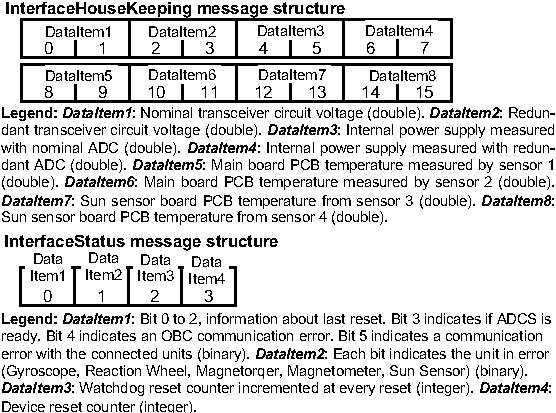
\includegraphics[width=8.4cm]{damat/images/BufferStructuresSmall}
		\caption{Structure of data buffers in \ESAIL.}
		\label{fig:appr:bufferStructure}
	\end{figure}
	
	% !TEX root = ../MAIN-DataDrivenMutationAnalysis.tex


\begin{table*}[tb]
\caption{Data-driven mutation operators}
\label{table:operators}
\scriptsize
\begin{tabular}{|p{40mm}|p{90mm}|}
\hline
\textbf{Fault Class}&\textbf{Description}\\
\hline
Value above threshold (VAT)&
Replaces the current value with a value above the threshold T for a delta (\D). 
\\
\hline
Value below threshold (VBT)&
Replaces the current value with a value below the threshold T for a delta (\D). 
\\
\hline
Value out of range (VOR)&
Replaces the current value with a value out of the range $[MIN;MAX]$.\\
\hline
Bit flip (BF)&
A number of bits randomly chosen in the positions between MIN and MAX are flipped.
\\
\hline
Invalid numeric value (INV)&
Replace the current value with a mutated value that is legal (i.e., in the specified range) but different than current value. 
\\
\hline
Illegal Value (IV)
&
Replace the current value with a value that is equal to the parameter \emph{VALUE}. 
\\
\hline
Anomalous Signal Amplitude (ASA)
&
The mutated value is derived by amplifying the observed value by a factor \emph{V} and by adding/removing a constant value \D from it. 
\\
\hline
Signal Shift (SS)
&
The mutated value is derived by adding a value \D to the observed value. 
\\
\hline
Hold Value (HV)
&
This operator keeps repeating an observed value for $V$ times. It emulates a constant signal replacing a signal supposed to vary.
\\
\hline
Fix value above threshold (FVAT)&
In the presence of a value above the threshold, it replaces the current value with a value below the threshold T for a delta \D. 
\\
\hline
Fix value below threshold (FVBT)&
It is the counterpart of FVAT for the operator VBT.
\\
\hline
Fix value out of range (FVOR)&
In the presence of a value out of the range  $[MIN;MAX]$ it replaces the current value with a random value within the range. 
\\
\hline
\end{tabular}
\end{table*}%

\clearpage

%\begin{figure}
%	\centering
%		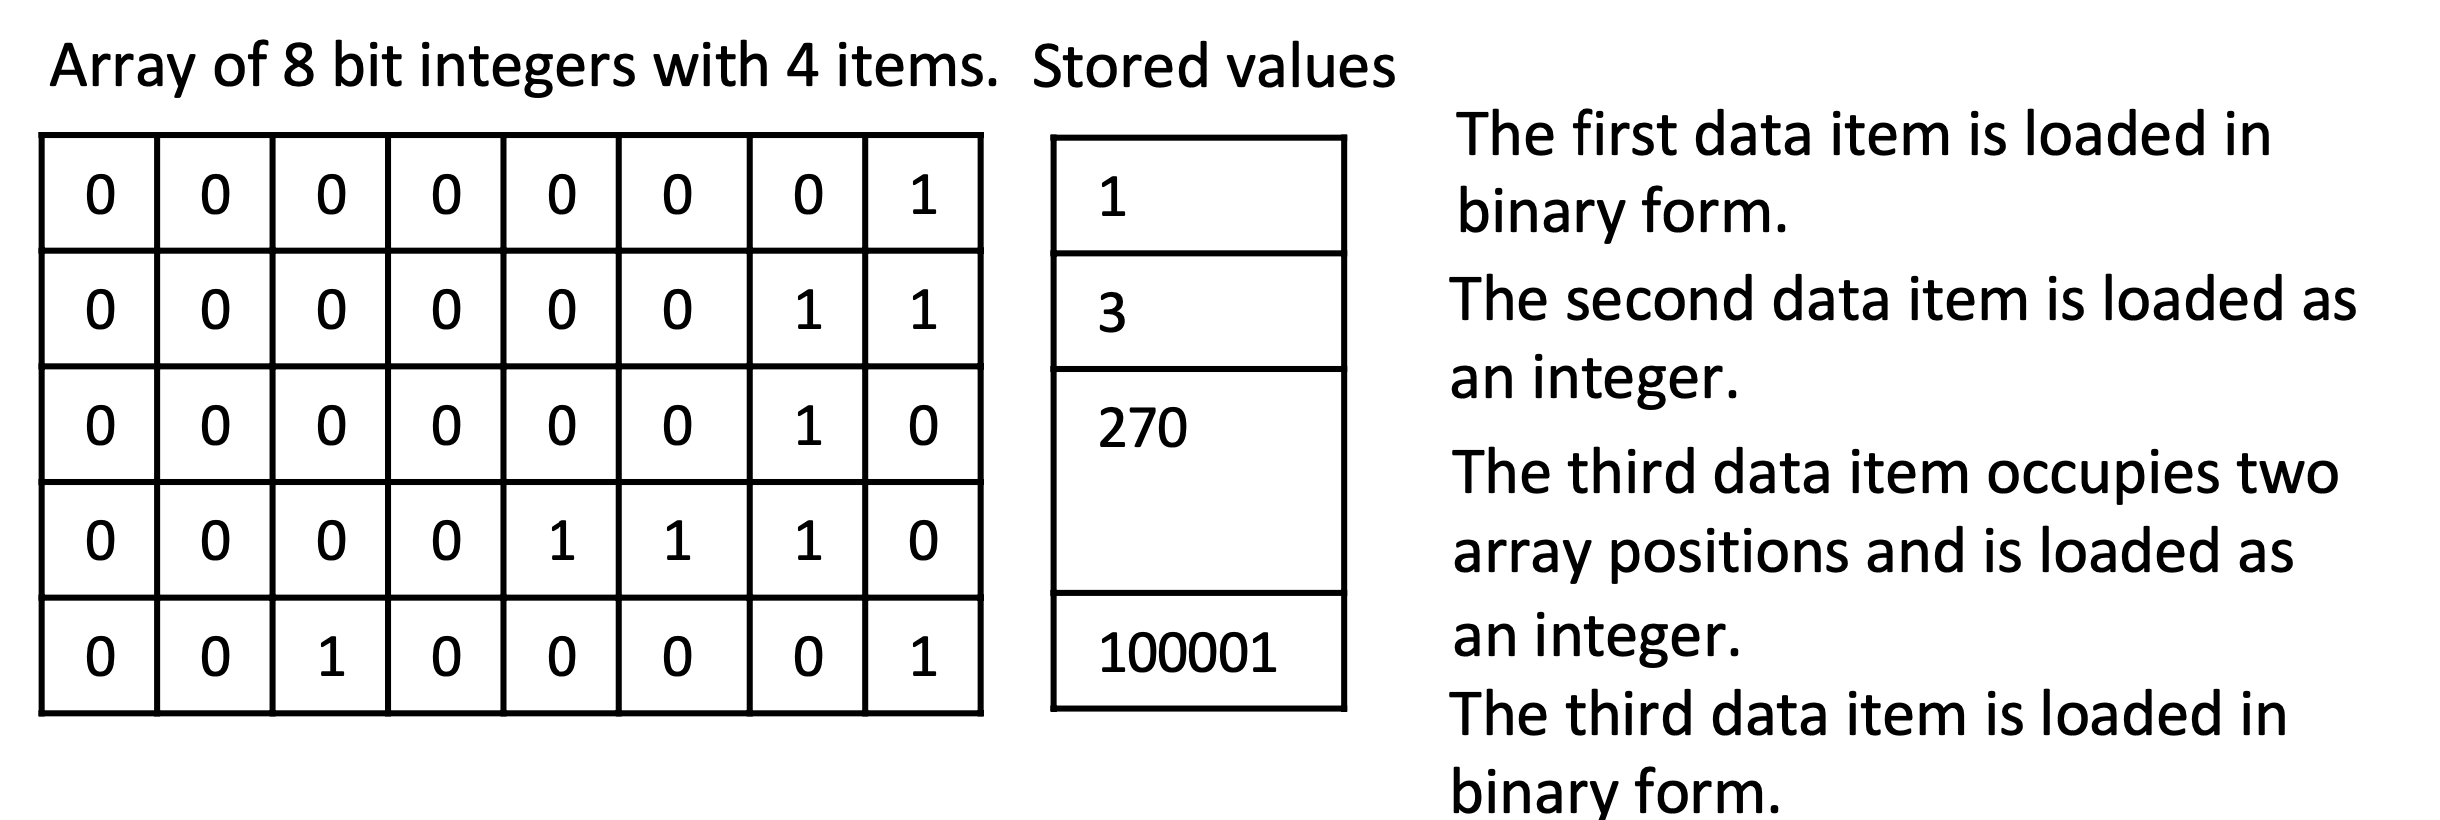
\includegraphics[width=8cm]{damat/images/bufferExample}
%		\caption{Example of a data buffer. \TODO{UPDATE PICTURE}}
%		\label{fig:appr:buffer}
%	\end{figure}

\subsubsection{Fault Modelling Methodology (Step 1)}
\label{sec:methodology}

% !TEX root =  ../MAIN-DataDrivenMutationAnalysis.tex

%
%\setlength\LTleft{0pt}
%\setlength\LTright{0pt}
%\begin{longtable}{@{\extracolsep{\fill}}|p{2.5cm}|p{5cm}|p{5cm}|@{}}
%\toprule


\begin{table}[tb]
\caption{\APPR fault modelling methodology}
\label{table:method}
\center
\scriptsize
\begin{tabular}{|
@{\hspace{1pt}}>{\raggedleft\arraybackslash}p{10mm}@{\hspace{1pt}}|
@{\hspace{1pt}}>{\raggedleft\arraybackslash}p{15mm}@{\hspace{1pt}}|
@{\hspace{1pt}}>{\raggedleft\arraybackslash}p{15mm}@{\hspace{1pt}}|
@{\hspace{1pt}}>{\raggedleft\arraybackslash}p{10mm}@{\hspace{1pt}}|
@{\hspace{1pt}}>{\raggedleft\arraybackslash}p{13mm}@{\hspace{1pt}}|
@{\hspace{1pt}}>{\raggedleft\arraybackslash}p{17mm}@{\hspace{1pt}}|
}
\hline
\textbf{Data} \textbf{nature}&\textbf{Representation} \textbf{type}&\textbf{Dependencies}&\textbf{\# of input} \textbf{partitions}&\textbf{Operators}&\textbf{Comments}\\
\hline
numerical&I, L, F, D&stateless/stateful&2&[VAT,FVAT]&Nominal below T\\
&&&&or [VBT,FVBT]&Nominal above T\\
\cline{4-6}
&&&3 or more&[VOR,FVOR]&\\
\cline{3-6}
&&stateful&&INV&For valid range\\
\cline{4-6}
&& &&[VOR,FVOR]&For out of range\\
\cline{3-6}
&&signal&&ASA, SS, HV&\\
\hline
categorical&I, H&N/A&N/A&IV&\\
\cline{2-6}
%&string&N/A&N/A&BF\\
%\cline{2-5}
&B&N/A&N/A&BF&\\
\hline
ordinal&I, H&N/A&N/A&ASA&\\
\hline
other&B&N/A&N/A&BF&\\
\hline
\end{tabular}\\
\textbf{Legend:} N/A not applicable.
\end{table}
%\normalsize

The fault model shall enable the specification of 
all possible interoperability problems in the SUT while minimizing equivalent and redundant mutants.
Equivalent mutants have the same observable output as the original SUT. 
Instead, redundant mutants have the same observable output as other mutants.
We use the term \INDEX{observable output} to refer to any output that can be verified by the test suite.
The equivalent or redundant nature of a mutant depends
on the equivalence relation for observable outputs
(i.e., how to determine if two outputs are the same).
In a testing context, such equivalence relation depends on the type of testing being performed. For example, system test cases, different than unit test cases,  are unlikely to verify the values of all the state variables of the system and thus mutants that are nonequivalent for unit test suites might be considered equivalent for system test suites. 
For example, in satellite systems, the correctness of the GPS triangulation algorithm output is verified by unit test cases; system test cases, instead, verify 
if the software takes appropriate actions when the satellite is out of orbit. Consequently, slight changes in the coordinates communicated by the GPS component may not lead to any change in the observable output verified by the test suite.
%When defining a fault model, engineers shall thus select and configure mutation operators in such a way that the mutations performed trigger changes in the observable output of the SUT (to avoid equivalent mutants) and (2) distinct mutations do not lead to the same observable outputs (to avoid redundant mutants).


We provide a set of guidelines for the definition of fault models that 
are summarized in Table~\ref{table:method}. 
For guidance,
% are based on the characteristics of the data being exchanged by CPS components.
we account for the nature of the data (i.e., numerical, categorical, ordinal, or binary) and their representation type.
Also, for numerical data, 
we consider 
%the type of measurement, that is, if the data is counted (i.e., it is discrete) or measured (i.e., it is continuous) and
%For numerical data, mutations shall be defined taking into consideration
the data dependencies, that is how data values depend on the previously observed values; we identified three categories: stateless (i.e., there are no dependencies between consecutive values), stateful (i.e, values depend on previous ones), and signal (i.e., values derive from a function of independent variables like time).
\CHANGED{Data dependencies determine the granularity of the mutation (i.e., with data dependencies, small differences shall be noticed); for non numerical data, we do not provide mutation operators with different granularities and data dependencies can be ignored.}
%on previous values and the time in which they are observed).

 

For \INDEX{stateless numerical data}, our guidelines are driven by input space partitioning concepts~\cite{Ammann:Offutt:2008}.
Indeed, given equivalence relations among outputs, it is unlikely that every change in \INDEX{stateless numerical data} will result into nonequivalent mutants; however, we can partition the input domain into regions with equivalent values (partitions).
Precisely, we rely on the  
\INDEX{interface-based input domain modeling} approach~\cite{Ammann:Offutt:2008}:
%Within data-driven mutation analysis, 
for each data item we identify a number of input partitions (set of values or value ranges) according to the interface specifications of the interacting components.
%each data item represents an input partition that shall be split into sets of values (or value ranges) identified according to the interface specifications of the interacting components.
%an input partition corresponds to a single data item and it shall be split into a set of blocks defined according to the interface specifications of the interacting components. 
In our methodology, the number and type of mutation operators selected for stateless numerical data depend on the number of input partitions identified.
With \emph{two input partitions} (e.g., nominal and exceptional data values), engineers can rely either on the pair [VBT,FVBT] or the pair [VAT,FVAT]. 
%Engineers shall select the pair of operators that simplifies the reading of the fault model.
%FABRIZIO: initially, I have explained what I mean with simplyfiy the reading (see below), however, these are details that may not be that necessary in a 10 pages conference paper.
%Engineers shall select the pair of operators that simplifies the reading of the data model; precisely, when the two input partitions capture  ranges for nominal and exceptional data values, the selection depends on how exceptional cases are identified (i.e., below or above the threshold). For other cases (i.e., two input partitions not related to exceptional cases), engineers can select any of the two pairs.
With \emph{three partitions}, engineers must configure one VOR and one FVOR operator. If a different delta (\D) is considered for the upper and lower bounds, engineers may configure two pairs [VBT,FVBT] and [VAT,FVAT], for the lower and upper bound, respectively. In the presence of \emph{more than three} partitions, engineers shall configure one [VOR,FVOR] pair for each extra partition above three (e.g., two pairs in the case of five partitions). The parameter \D{} is used to determine the partition to which the mutated data belongs. 
%Please note that mutants belonging to each pair shall not lead to redundant mutants.
%Engineers can configure multiple [VOR,FVOR] pairs in case several combinations needs to be tested.


In the presence of \INDEX{stateful data}, replacement with random values in the valid range (i.e., the INV operator) will lead to nonequivalent mutants (e.g., because it leads to data values that are systematically different than the values expected for the current system state). Alternatively, the valid data range might be partitioned as for stateless data. However, to avoid redundant mutants, engineers should rely either on the INV operator or the partitioning of the valid data range. 
The effect of data outside the valid data range should instead be verified by means of the [VOR, FVOR] pair.

For \INDEX{signal values}, depending on the shape of the expected signal, engineers should configure one operator among the ASA, SS, and HV. The configuration of more than one of these operators may lead to redundant mutants (e.g., because each of them triggers the same warning in the SUT).

With \INDEX{categorical data} represented using \emph{integers and hexadecimals}, engineers must configure one IV operator for each possible value; indeed, a change in the observed category shall trigger a different behaviour in the SUT. 
%With categorical data represented using labels (e.g., strings), engineers shall configure one BF operator with the MAX parameter set to the minimum number of characters taken by the string; indeed, such a bit flip mutation ensures to alter the transmitted label (e.g., change a characater of the string label) and thus introduce a nonequivalent mutant.
With categorical data in \emph{binary form}, each bit indicates a specific class (e.g., the unit in error for the DataItem2 in the IFStatus message of Figure~\ref{fig:appr:bufferStructure}).  
To verify that the test suite can detect any possible category change, engineers must configure two BF operators for every bit (both MIN and MAX must coincide with the bit position), one operator must flip a bit when it is set (i.e., $\mathit{STATE}=1$), and the last one when it is unset (i.e., $\mathit{STATE}=0$). 
%If only two categories are represented by the data item (i.e., only one bit is used), it is sufficient to configure one BF operator.

For \INDEX{ordinal data}, which is represented by means of either integers or hexadecimals, we suggest to apply the ASA operator with \emph{T} being set to the middle point of the ordinal scale and \D set to the step distance between consecutive data (usually $1$). For data in binary form (e.g., pictures), engineers must configure a BF operator to flip a number of bits  that is sufficient to alter the semantics of the data (e.g., introduce sufficient noise in images).

%, and values are selected from each region.
%
%==> the structure of the input domain in terms of input characteristics. The test engineer creates a partition for each characteristic. The partition is a set of blocks, each of which contains a set of values. From the perspective of that particular characteristic, the values in each block are considered equivalent.



%observable output difference.
%For stateless data, changes in the observable output of the SUT shall be expected when a data item value is replaced with a data item value that belongs to a differ
%
%For visible output we refer to any (e.g., two mutants causing the same failures in the test suite).
%
%We have an equivalent mutant..
%In system and integration test suites (i.e., the ones exercising components interoperability) it is unlikely that any change in the data exchanged by components result in a test case failure. 
% 
%
%Somehow, to make a system test case fail, the granularity of the error observed the data shall be coarser than the one require to make a unit test case fail. In a mutation analysis context this means that, to avoid equivalent mutants (that is 
%
%targeting functional correctness of the results computed after processing
%
%and thus make test cases fail.

% !TEX root = ../MAIN.tex
\begin{table}[h]
\begin{center}
\scriptsize
\begin{tabular}{|p{2cm}|p{2cm}|p{4cm}|p{6cm}|}
\hline
\textbf{Fault Class}&\textbf{Types}&\textbf{Parameters}&\textbf{Description}\\
\hline
Value above threshold (VAT)&
\begin{minipage}{6cm}
INT\\
LONG INT\\
FLOAT\\
DOUBLE
\end{minipage}
&
\begin{minipage}{6cm}
T: threshold\\
D: delta with respect to threshold\\
\end{minipage}
&
\begin{minipage}{6cm}
The value is above a threshold T for a delta D. 

\EMPH{Data mutation operation:} The mutation is performed by replacing the current value (a number) with a value of the same type that is equal to $(T+D)$.
\end{minipage}
\\

\hline
Value below threshold (VBT)&
\begin{minipage}{6cm}
INT\\
LONG INT\\
FLOAT\\
DOUBLE
\end{minipage}
&
\begin{minipage}{6cm}
T: threshold\\
D: delta with respect to threshold\\
\end{minipage}
&
\begin{minipage}{6cm}
The value is below a threshold T for a delta D. 

\EMPH{Data mutation operation:} The mutation is performed by replacing the current value (a number) with a value of the same type that is equal to $(T-D)$.
\end{minipage}
\\



\hline
Value out of range (VOR)&
\begin{minipage}{4cm}
INT\\
LONG INT\\
FLOAT\\
DOUBLE
\end{minipage}
&
\begin{minipage}{4cm}
MIN: minimum valid value\\
MAX: maximum valid value\\
D: delta with respect to minimum/maximum valid value
\end{minipage}
&
\begin{minipage}{6cm}
The value is out of the valid range MIN-MAX. 

\EMPH{Data mutation operations (2):}  The mutation is performed by replacing the current value (a number) with 
\begin{itemize}
\item a value of the same type that is equal to $(MIN-D)$
\item a value of the same type that is equal to $(MAX+D)$
\end{itemize}
\end{minipage}
\\

\hline
Bit flip (BF)&
BIN
&
\begin{minipage}{4cm}
MIN: lower bit\\
MAX: higher bit\\
STATE: mutate only if the bit is in the given state\\
\TRFOUR{VALUE: integer specifying the number of bits to mutate}\\
\end{minipage}
&
\begin{minipage}{6cm}
A number of bits randomly chosen in the positions between MIN and MAX (included) are flipped.

\EMPH{Data mutation operation:} the operator flips N randomly selected bit.
If STATE is specified, the mutation is applied only if  the bit is in the specified state. Parameter VALUE specifies the number of bits to mutate.
\end{minipage}
\\

\hline
Invalid numeric value (INV)&
\begin{minipage}{6cm}
INT\\
LONG INT\\
FLOAT\\
DOUBLE
\end{minipage}
&
\begin{minipage}{4cm}
MIN: lower valid value\\
MAX: higher valid value\\
\TRFOUR{D: distribution to follow}\\
\TRFOUR{VALUE: mean value for normal distribution}\\
\end{minipage}
&
\begin{minipage}{6cm}
The value is legal (i.e., in the specified range) but different than the current one, which, in this case, is expected to be consistent with the status of the system.

\EMPH{Data mutation operation:} Mutation is performed by replacing the current value with a different value randomly sampled in the specified range. The parameter D specified the distribution to follow when performing the mutation\footnote{In our implementation 0 indicates uniform, 1 indicates normal around the specified value (but in range).}
\end{minipage}
\\

\hline
Illegal Value (IV)
&
\begin{minipage}{6cm}
INT\\
LONG INT\\
FLOAT\\
DOUBLE
\end{minipage}
&
\begin{minipage}{6cm}
VALUE: illegal value that is observed\\
\end{minipage}
&
\begin{minipage}{6cm}
The value is illegal and equal to the provided one (i.e., parameter \emph{VALUE}).

\EMPH{Data mutation operation:} Mutation is performed by replacing the current value with the value \emph{VALUE}, if different than the current one.
\end{minipage}
\\

\hline
\TRFOUR{Anomalous Signal Amplitude (ASA)}
&
\begin{minipage}{6cm}
INT\\
LONG INT\\
FLOAT\\
DOUBLE
\end{minipage}
&
\begin{minipage}{6cm}
T: change point\\
D: delta to add/remove\\
V: value to multiply\\
\end{minipage}
&
\begin{minipage}{6cm}
The value is modified by amplifying/reducing it by a factor V and adding or removing D from the observed value. It is used to "amplify" a signal in a constant manner to simulate unusual signal. T indicates the observed value below which instead of adding  we subtract .

\EMPH{Data mutation operation:} Mutation is performed by replacing the current value ($v$) with the value ($v'$) computed as follows:

\[
v' =  
    \begin{cases}
      T+(  (v-T)*V  ) + D   & \mathit{if}\ v \ge T\\
      T - (  (T-v)*V  ) - D   & \mathit{if}\ v < T
    \end{cases}       
\]
\end{minipage}
\\


\hline
\TRFOUR{Signal Shift (SS)}
&
\begin{minipage}{6cm}
INT\\
LONG INT\\
FLOAT\\
DOUBLE
\end{minipage}
&
\begin{minipage}{6cm}
D: delta by which the signal should be shifted\\
\end{minipage}
&
\begin{minipage}{6cm}
The value is modified by adding a value D. It simulate an anomalous shift in the signal.
\end{minipage}
\\





\hline
\TRFOUR{Hold Value (HV)}
&
\begin{minipage}{6cm}
BIN\\
INT\\
LONG INT\\
FLOAT\\
DOUBLE
\end{minipage}
&
\begin{minipage}{6cm}
V: number of times to repeat the same value\\
\end{minipage}
&
\begin{minipage}{6cm}
This operator keeps repeating an observed value for $V$ times. It emulates a constant signal replacing a signal supposed to vary.
\end{minipage}
\\



\hline
\TRFOUR{Array Swap (AS)}
&
\begin{minipage}{6cm}
ARRAY\_*\\
\end{minipage}
&
\begin{minipage}{6cm}
MIN: position of element A\\
MAX: position of element B\\
VALUE: number of elements to move\\
\end{minipage}
&
\begin{minipage}{6cm}
Replace a number of elements (number specified by VALUE) located starting from position MIN, with a number of elements located starting from position MAX, and viceversa.
\EMPH{Data mutation operation:} Mutation is performed by replacing the two set of elements with each other.
\end{minipage}
\\


\hline
\TRFOUR{Array Random Swap (ARS)}
&
\begin{minipage}{6cm}
ARRAY\_*\\
\end{minipage}
&
\begin{minipage}{6cm}
MIN: min position of element A/B\\
MAX: max position of element A/B\\
VALUE: number of elements to move\\
\end{minipage}
&
\begin{minipage}{6cm}
Replace a number of elements (number specified by VALUE) located in a position between MIN and MAX, with a number of elements located in a position between MIN and MAX. MIN and MAX specify a position with respect to the beginning and end of the array.  For example, MIN=0 indicates the first element of teh array, MIN=-2 indicates the second element of the array.
\EMPH{Data mutation operation:} Mutation is performed by replacing the two set of elements with each other.
\end{minipage}
\\



%Incorrect Identifier& Several transmission data fields have fixed values, for example fields identifying the transmitting satellite. Hardware/software errors may assign incorrect identifiers.\\
%%Incorrect Checksum& Hardware/software errors may result in an incorrect checksum for a Packet or VCDU.\\
%Incorrect Counter& Counters are used to track Packet or VCDU ordering. Hardware/software errors may assign incorrect counter values.\\
%Flipped Data Bits& Physical channel noise may flip one or more bits in the data transmission.\\
\hline
\end{tabular}
\end{center}
\caption{Data Fault Classes}
\label{table:faultModel:FAQAS}
\end{table}%

Table~\ref{table:faultModel} provides a specification in tabular form (i.e, the format processed by \APPR) of two fault models configured for the IfKH (i.e., Interface House Keeping) and IfStatus (i.e, Interface Status) messages. In the fault models, each row captures the configuration of a mutation operator for a specific data item. For example, row number 5 indicates that \APPR interprets as double the data inside the two buffer units starting at position 10 (units 10 and 11) and applies the VAT operator. Rows 1 and 2 show that, for a same numerical data item (i.e., the one covering units 8 and 9), we can apply both the VAT and VBT operators, using a different delta for each. 
Rows 2 and 4 show the FVAT and FVBT operators complementing the VAT and VBT operators in rows 1 and 3. They simulate the case in which data for the nominal cases is observed instead of data for exceptional cases, as visible in Table~\ref{table:operators}.
Rows 8 to 23 show that different bits of a same data item can be targeted by different BF operators. %Rows 12 to 14 concern binary categorical data with two categories each, which is the reason why we configured one BF with no STATE setting, according to our methodology. 
\UPDATED{Rows 8 to 13 concern binary categorical data with two categories each, thus we configured two BF each}. 
Rows 14 to 23 concern binary categorical data with five categories; consequently, they present ten BF operators configured for the five categories.
%of DataItem 1.




Figure~\ref{fig:dataMutationFMExamples} provides a visual representation of an array of 8 bit unsigned integers (i.e., unsigned chars) that is modelled using the \EMPH{FMExample} fault model in Table~\ref{table:faultModel:example}. It also provides an example of the mutated data generated by the six mutation operation instances derived from the fault model in Table~\ref{table:faultModel:example}.


% !TEX root = ../MAIN.tex
\begin{table}[h]
\begin{center}
\small
\begin{tabular}{|p{1cm}|p{2cm}|p{1cm}|p{1cm}|p{1cm}|p{1cm}|p{1cm}|p{2cm}|p{1cm}|p{1cm}|}
\hline
\textbf{Fault Model Name}&\textbf{DataItem}&\textbf{Span}&\textbf{Type}&\textbf{Fault Class}&\textbf{Min}&\textbf{Max}&\textbf{Threshold}&\textbf{Delta}&\textbf{State}\\
\hline
IfHK&0&1&BIN&BF&0&0&-&-&-\\
IfHK&1&1&INT&VOR&0&5&-&1&-\\
IfHK&2&2&BIN&BF&0&63&-&-&-\\
IfHK&4&1&BIN&BF&0&0&-&-&-\\
\hline
IfStatus&0&1&BIN&BF&0&0&-&-&-\\
\hline
\end{tabular}
\end{center}
\caption{Driven Fault Model Buffer}
\label{table:faultModel:example}
\end{table}%

\begin{figure}[h]
  \centering
    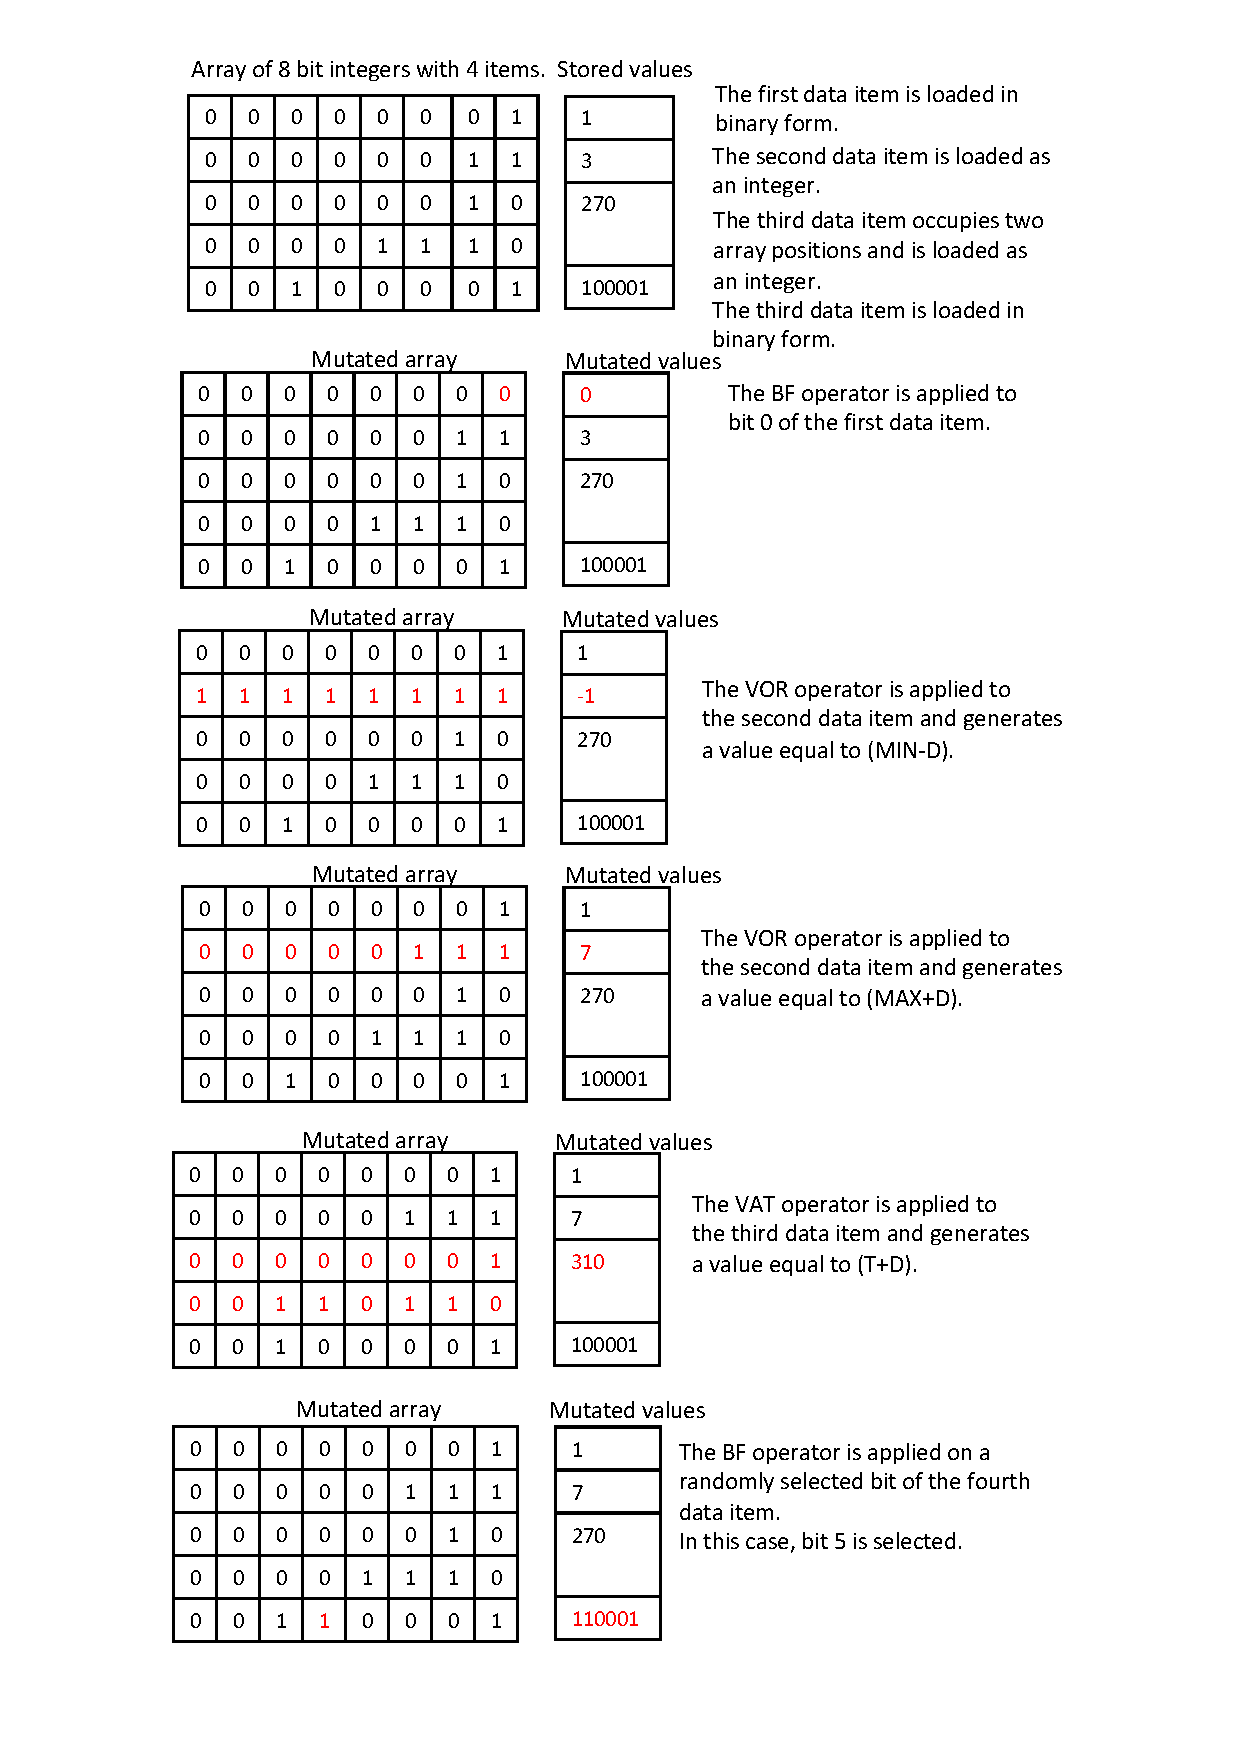
\includegraphics[width=12cm]{images/dataMutationFMExample.pdf}
      \caption{Example of original data and  data mutated according to the fault model in Table~\ref{table:faultModel:example}.}
      \label{fig:dataMutationFMExamples}
\end{figure}





\clearpage


\subsubsection{Automated Generation of Mutation API (Step 2) and Probe Insertion (Step 3)}
\label{sec:generateAPI}

\begin{figure}[tb]
\centering
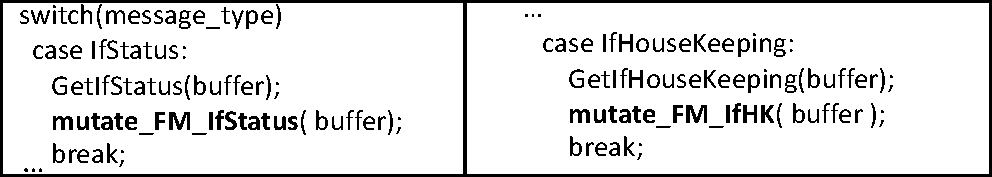
\includegraphics[width=7cm]{damat/images/ProbesExample}
\caption{Example of \APPR mutation probes (in bold).}
\label{fig:appr:ProbesExample}
\end{figure}

\APPR automatically generates a \INDEX{mutation API} to perform mutations at runtime. The API implements a set of functions (called \INDEX{mutate\_FM\_<name>}) that mutate a data buffer according to the given fault model. 
These functions select the data item to mutate and the mutation procedure to apply based on the mutant under test (see Section~\ref{sec:mutantsGeneration}). 

The \APPR mutation API works with C/C++ code; however it may be extended to deal with other programming languages.
Since it is not possible to automatically determine which data buffer to mutate, \APPR requires engineers to modify the source code of the CPS under test by introducing a mutation probe which consists of an invocation of the \APPR function that mutates the data buffer according to a specific fault model.
Note that the effort required by the engineer is minimal; indeed, the exchange of data between components is usually managed in a single location (e.g, the function that serializes the data buffer on the network) and thus it is usually sufficient to introduce one function call for each message type to mutate.
Figure~\ref{fig:appr:ProbesExample} shows how the implementation of \ESAIL has been modified to add the mutation probes. 
The SVF function was modified to handle the message requests sent to the ADCS by inserting one mutation probe for each message type to mutate, e.g., IfStatus and IfHouseKeeping in~Figure~\ref{fig:appr:ProbesExample}. 
Function \emph{mutate\_FM\_IfStatus} is part of the generated mutation API; it loads the fault model \emph{IfStatus} into memory (\UPDATED{our API relies on a tree data structure}) and then invokes the function \emph{mutate}. The function \emph{mutate} performs data-driven mutation according to the provided fault model; the implementation of \emph{mutate} is part of the \APPR toolset.



% At a high-level,
%function \emph{mutate} taking into account the size of the data item; it  checks if the 


The behavior of function \emph{mutate} depends on the value of a unique identifier (i.e., the \emph{MutantID}) associated at compile time to the mutant; the \emph{Mutant ID} univocally identifies the performed mutation operation (each mutant executes one mutation operation, see Section~\ref{sec:mutantsGeneration}).
At a high level, \emph{mutate} performs four activities. First, it checks if the mutation should be performed (i.e., if the data buffer is targeted by the mutation operation identified with the \emph{Mutant ID}). Second, it casts the data item instance targeted by the mutant to a support variable of the type specified in the fault model. Third, it mutates the data stored in the support variable; for each mutation operator, we have implemented a distinct set of instructions for each data representation type. Fourth, before terminating, the function \emph{mutate} writes the mutated data back to the data buffer.





\subsubsection{Automated Generation of Mutants (Step 4)}
\label{sec:mutantsGeneration}



Consistent with code-driven mutation analysis, \APPR generates one mutant for each mutation procedure of the mutation operators configured in the fault model. Each mutant performs exactly one \INDEX{data mutation operation} (i.e., a data mutation procedure configured for a specific data item). For example, the specification in row 6 of Table~\ref{table:faultModel} makes \APPR generate two mutants: each mutant modifies the value of the data item starting at position 12 but one mutant replaces the current value with the value 51 (i.e., $50+1$) while the other replaces the current value with the value $-21$ (i.e., $-20 -1$).

The mutant generation is invisible to the end-user who does not need to modify the source code further; indeed, we rely on a C macro to specify, at compile time, which mutation operation must be performed by every mutant. Mutants are generated by compiling the \UPDATED{SUT} multiple times, once for each mutation operation. At runtime, the mutate function executes only the mutation operation selected for the mutant under test.

\subsubsection{Mutants Execution (Step 5)}
\label{sec:mutantsExecution}

As for \INDEX{code-driven mutation analysis}, the test suite under analysis is executed iteratively with every data-driven mutant. 
At runtime, all the data items targeted by a mutant are mutated whenever the mutation preconditions hold (e.g., the STATE of the BF operator); we leave the mutation of a sampled subset of \UPDATED{data item instances to future work~\cite{zhang2013operator,gopinath2015hard}.}

To speed up the mutation analysis process, the test suite under analysis is first executed with a special mutant that, instead of mutating data items, keeps trace of the fault models loaded by each test case; in other words, it traces what are the data types covered by each test case. The collected information enables the execution, for every mutant, of the subset of test cases that cover the 
message type
%type of data 
targeted by the mutant, thus speeding up mutation analysis.


\subsubsection{Mutation Analysis Results (Step 6)}
\label{sec:mutationAnalysisResults}

Inspired by work on \INDEX{abstract mutation analysis}~\cite{Offutt2006}, we have defined three metrics to evaluate test suites with data-driven mutation analysis: \INDEX{fault model coverage}, \INDEX{mutation operation coverage}, and \INDEX{mutation score}. 
%The first two provide information about the quality of test inputs, whereas the latter provides information about the quality of test oracles \CHANGED{and the test process}. Different from code-driven mutation analysis, data-driven mutation analysis thus enables engineers to distinguish between these two distinct problems affecting test suite effectiveness.
These metrics measure the frequency of the following scenarios: (case 1) the message type targeted by a mutant is never exercised, (case 2) the message type is covered by the test suite but it is not possible to perform some of the mutation operations (e.g., because the test suite does not exercise out-of-range cases), (case 3) the mutation is performed but the test suite does not fail.
\CHANGED{Different from code-driven mutation analysis, these three metrics enable engineers to distinguish between possible test suite shortcomings, including untested message types, uncovered input partitions, poor oracle quality, 
%faulty software, 
and lack of test inputs.}

\INDEX{Fault model coverage (FMC)} is the percentage of fault models covered by the test suite. Since we define a fault model for every 
message type exchanged by two components,
%different data buffer (i.e., type of data exchanged by two components), 
it provides information about the extent to which the message types actually exchanged by the SUT are exercised and verified by the test suites. 
%In other words, low fault model coverage indicates that many test scenarios (e.g., a specific sequence of test inputs being sent to the CPS when the environment is in a specific state) are not exercised by a test suite. 
\CHANGED{Since different component functionalities often require different message types, low fault model coverage may indicate that only a small portion of the integrated functionalities have been tested.}

\INDEX{Mutation operation coverage (MOC)} is the percentage of data items that have been mutated at least once, considering only those that belong to the data buffers covered by the test suite. It provides information about the input partitions covered for each data item; for example, the FVOR operator leads to two mutation operations, which are applied only if the observed value is outside range. Otherwise the two mutation operations will not be covered, thus enabling the engineer to identify such shortcoming in the test suite.
%TODO: add example

The \INDEX{mutation score (MS)} is the percentage of mutants killed by the test suite \UPDATED{(i.e., leading to at least one test case failure)} among the mutants that target a fault model and for which at least one mutation operation was successfully performed. It provides information about the quality of test oracles; indeed, a mutant that performs a mutation operation and is not killed (i.e., is \emph{live}) indicates that the test suite cannot detect the effect of the mutation (e.g., the presence of warnings in logs).
% or an unexpected output from the system). 
\CHANGED{Also, a low mutation score may indicate missing test input sequences. Indeed, live mutants may be due to either software faults (e.g., the SUT does not provide the correct output for the mutated data item instance) or the software not being in the required state (e.g., input partitions for data items are covered when the software is paused); in such cases, with appropriate input sequences, the  test suite would have discovered the fault or brought the SUT into the required state. Both poor oracles and lack of inputs indicate flaws in the test case definition process (e.g., the stateful nature of the software was ignored).}

\clearpage
\subsection{Running Examples}
\label{sec:dataDriven:example}

In this Section, we provide a set of running examples that show the results achieved by \APPR in the presence of test suites affected by different problems. More precisely we aim to demonstrate, for representative cases, the absence of false alarms due to equivalent mutants and the usefulness of the mutation analysis metrics computed. 
\REVTOOL{P-3}{Each running example is an artificial but realistic definition of test suites to illustrate the methodology.}
We consider the following representative scenarios:
\begin{enumerate}
\item The test suite exercises only one message exchange between the ADCS and the SUT; each test case covers a distinct input partition.
\item The test suite exercises only one message exchange between the ADCS and the SUT; multiple test cases cover a same input partition.
\item The test suite exercises multiple message exchanges between the ADCS and the SUT; each test case covers a distinct combination of input partitions.
\end{enumerate}


\subsubsection{Example set 1: One message exchange, distinct input partitions}
\label{sec:dataDriven:example:1}

\begin{figure}[tb]
\centering
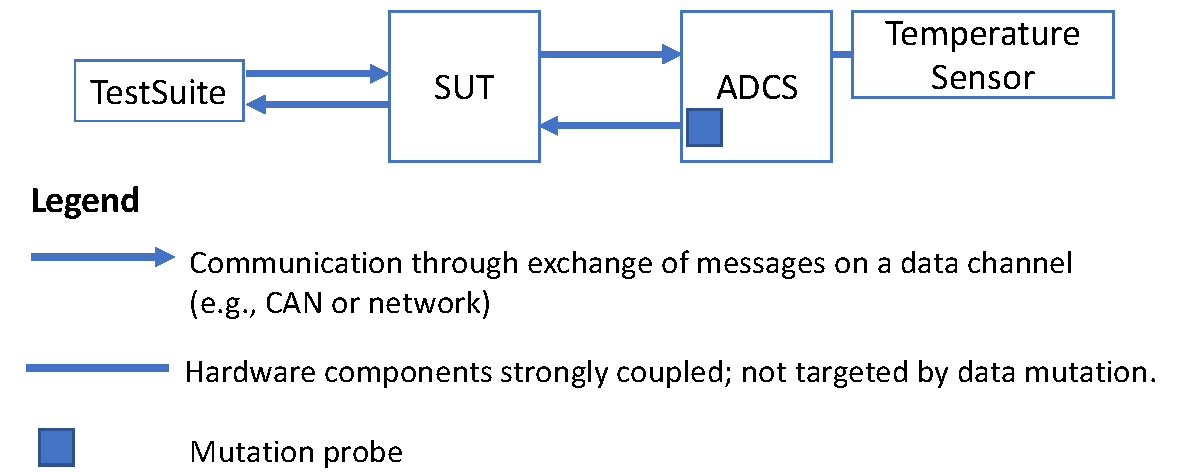
\includegraphics[width=8cm]{damat/RunningExampleArch}
\caption{Architecture of the running example system.}
\label{fig:damat:RunningExampleArch}
\end{figure}

Our first set of running examples concerns the presence of a single message exchange and test cases covering distinct input partitions.

Our examples concern an SUT that exchanges with the ADCS component one type of message. More precisely, the ADCS sends a message (hereafter, \emph{TempMessage}) with the temperature collected by its sensor. The architecture of such system is shown in Figure~\ref{fig:damat:RunningExampleArch}. For simplicity, we assume that the ADCS periodically sends a TempMessage to the SUT. The ADCS is connected to the TemperatureSensor. The communication between the ADCS and the TemperatureSensor is not affected by data-driven mutation. We may assume the ADCS and the TemepratureSensor are simulated during the execution of the test suite. The SUT and the ADCS communicate through a channel 
(e.g., a CAN bus). The data mutation probe is inserted in the ADCS simulator; in practice we mutate the data generated by the ADCS. The test suite exercises the software under test by communicating through a data channel; the type of communication channel used by the test suite is not relevant for the purpose of the running example.

For our running example, the SUT has two state variables that are observable by the test suite, \emph{temperature} and \emph{temperature\_alarm}. The state variable \emph{temperature} reports the temperature returned by the sensor in the last message. 
The state variable \emph{temperature\_alarm} is set to 1 if the temperature returned by the sensor is above 100.

The test suite is comprised of two test cases. \emph{Test 1} exercises the SUT with a temperature in the nominal case (i.e., temperature below 100), \emph{Test 2} concerns the non nominal case (i.e., temperature above 100). The two test cases of the test suite exercise the same sequence of interactions, which are depicted in the UML Sequence diagram of Figure~\ref{fig:damat:RunningExample1Sequence}. The sequence diagram shows that the test case first starts the ADCS simulator and the SUT; then, it waits for the ADCS to send the TempMessage before requesting the values of the variables \emph{temperature} and \emph{temperature\_alarm}. Figure~\ref{fig:damat:RunningExample1Sequence} also shows that, in this case, the mutation is performed within the ADCS simulator.

\begin{figure}[tb]
\centering
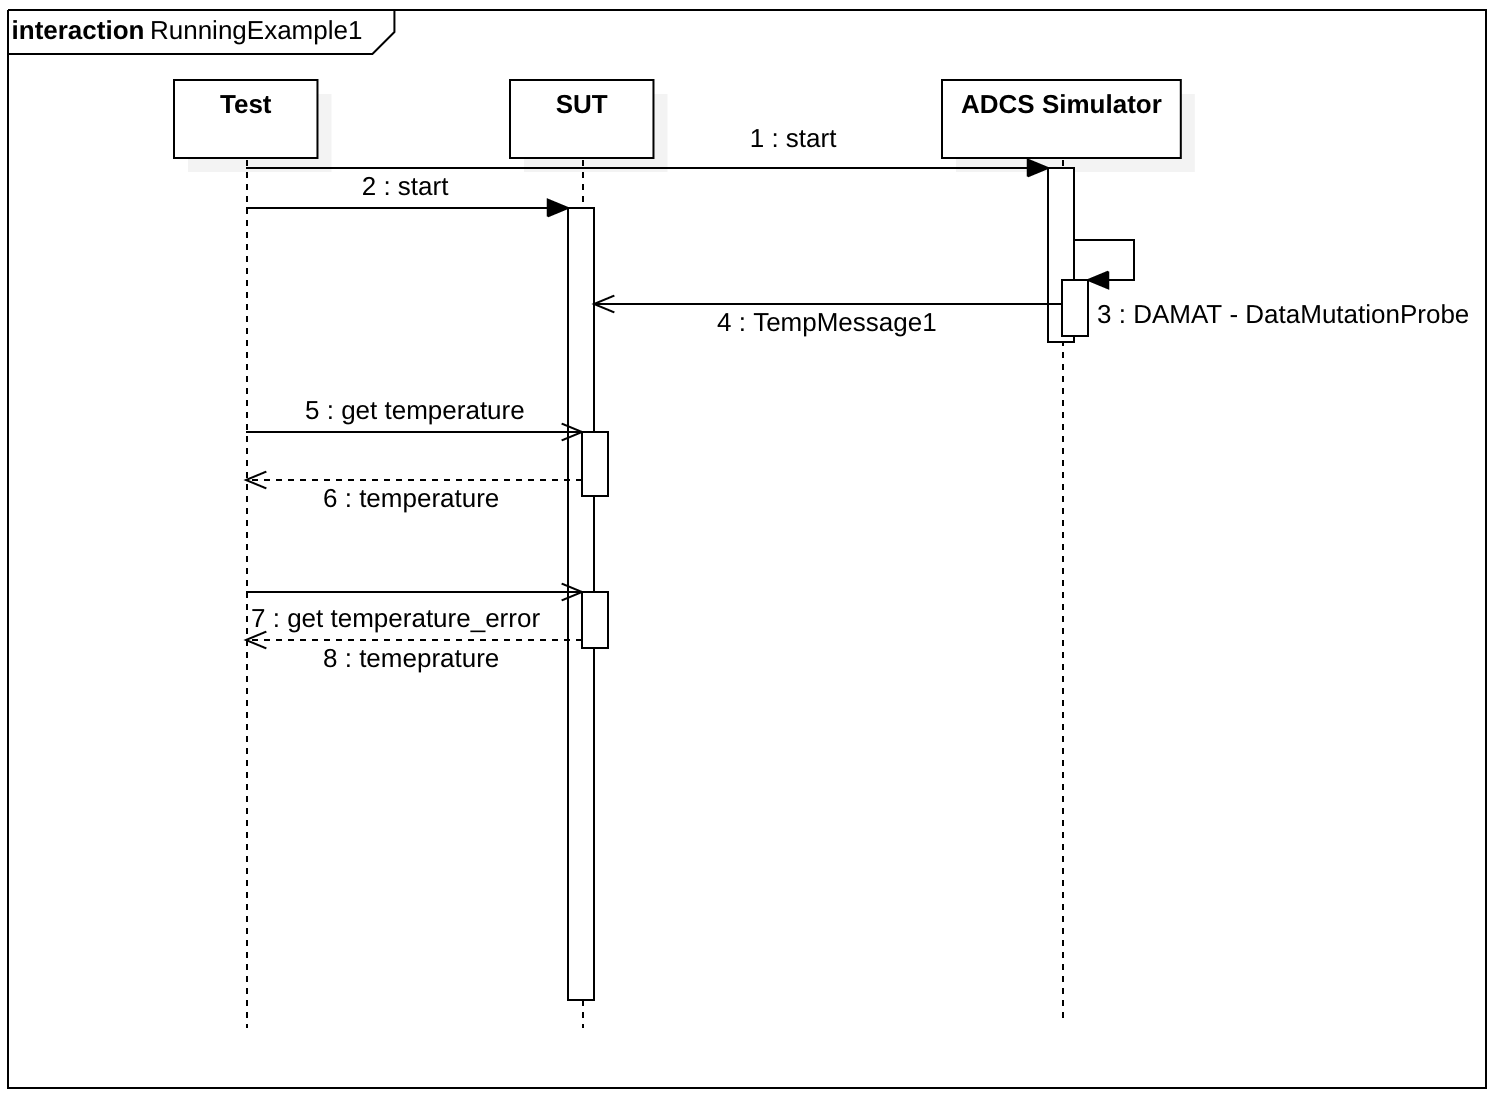
\includegraphics[width=8cm]{damat/images/runningExamplesSequence1.png}
\caption{Interactions exercised by the test cases belonging to the running example set 1.}
\label{fig:damat:RunningExample1Sequence}
\end{figure}


Figures~\ref{fig:damat:RunningExample1A} to~\ref{fig:damat:RunningExample1C} show our running examples. On the top, we report the fault model. In this case the fault model applies the operators VAT (value above threshold) and FVAT (fix value above threshold). The VAT operator is configured with a threshold of 100 and a delta of 10 (i.e., it replaces values below the threshold with the value 110). The FVAT operator is configured in the same manner (i.e., it replaces values above threshold with the value 90). The operator VAT leads to \emph{MUTANT 1}, the operator FVAT leads to \emph{MUTANT 2}; \REVTOOL{P-5}{to summarize, in this example we have two mutants, each implements one distinct mutation operator.}

In Figure~\ref{fig:damat:RunningExample1A}, under \emph{Exchanged data}, we report the sequence of data messages exchanged by the test cases of the test suite (one column for each test case).
In the following rows, we report the oracles. For each oracle we indicate how it verifies if a state variable has been assigned with a correct value; we indicate $"=="$ if it verifies the exact value taken by the state variable (e.g., \emph{temperature == 50)}, "$>=$" if it verifies that the value is above a threshold (e.g., \emph{temperature $>=$ 50}). Please note that, according to standard practice, test cases for non nominal cases verify that state variables contain the expected alarm and anomalous values (i.e., the test case passes only if the SUT report the anomaly). 

For each mutant, we report the value of the data exchanged during the execution and the data of the state variables read by the oracle. In red we indicate data that has been mutated according to the fault model. 
If an oracle does not read the value of a variable we leave the cell empty.
Failing oracles are highlighted in yellow.
\REVTOOL{P-5}{Note that for each mutant we provide multiple columns (named \emph{Test 1} and \emph{Test 2}), each provides the data exchanged during the execution of the test case.}
Finally, for each mutant, for each oracle, we report the test cases that detect the anomalous value (if any); also, we report if the mutant had been killed.


Please note that, following the \APPR procedures, MUTANT 1 does not mutate the data exchanged by Test 2 because it is already above the threshold. MUTANT 2 does not mutate the data exchanged by Test 1 because it is already below the threshold.

TestSuite1 is an optimal test suite that verifies the expected value of all the state variables. For MUTANT 1, Test 1 fails because the assertion about temperature fails (expected 50 observed 110).
For MUTANT 2, Test 2 fails because the assertion about temperature fails (expected 120 observed 90).
\REVTOOL{P-6}{We have a fault model coverage (\emph{FMC}) of 100\% because we have only one fault model and it is covered (i.e., the test suite exchanged the data message under analysis). We have a mutation operator coverage (\emph{MOC}) of 100\% because all the mutation operations associated with the configured mutation operators are applied (in other words, all the mutants perform at least one mutation of a data item instance). We have a mutation score (\emph{MS}) of 100\% because, for each mutant, at least one test case fails.}

TestSuite2 verifies the expected value of the temperature for the nominal case and the presence of a temperature error for the non nominal case. For MUTANT 1, Test 1 fails because the assertion on temperature fails (expected 50 observed 110).
For MUTANT 2, Test 2 fails because the assertion on temperature errors fail (expected 1 observed 0).
\REVTOOL{P-6}{Concerning FMC, MOC, and MS, the same considerations made for TestSuite1 hold.}

TestSuite3 verifies only temperature values while TestSuite4 verifies only temperature alarms. They all kill the mutants for the same reasons reported in the cases above. \REVTOOL{P-6}{Concerning FMC, MOC, and MS, the same considerations made for TestSuite1 hold.}


TestSuite5 is a copy of TestSuite2 having an imprecise oracle (i.e., it verifies that temperature is above 50 instead of equal to 50). Consequently the test suite does not fail for MUTANT 1 and the mutation score is not 100\%; consequently, \APPR enables an engineer to detect the limitation of the test suite.

\REVTOOL{P-6}{TestSuite6} is a copy of TestSuite2 without an oracle for Test2 (i.e., it does not verify the presence of temperature alarms). Consequently, the test suite does not fail for MUTANT 2 and the mutation score is not 100\%; consequently, \APPR enables an engineer to detect the limitation of the test suite.

TestSuite7 is a copy of TestSuite2 with multiple test cases covering the same input partitions; indeed, Test3 covers the same input partition of Test1 (i.e., it exercises the value 0, which is a nominal value like 50), Test4 covers the same input partition of Test2 (i.e., it exercises the value 101, which is a non nominal value like 120). All the mutants are killed by the test suite and we do not observe equivalent mutants.

TestSuite8 is a copy of TestSuite7 with the same limitations of TestSuite6 (i.e., Test2 does not contain an oracle).
In this case, the mutation score is 100\% because Test 4 contains an appropriate oracle and covers the same input partition not appropriately verified by Test 2. We do not observe equivalent mutants.

TestSuite9 is a copy of TestSuite7 without oracles for both Test2 and Test4; similarly to the case of TestSuite6, since the non-nominal partition is not appropriately verified, the mutation score is not 100\%; consequently, \APPR enables an engineer to detect the limitation of the test suite.

TestSuite10 covers the case of a test suite that does not exercise an input partition; precisely, it does not exercise non nominal values. 
In this case, \APPR can detect that MUTANT 2 is never applied (to exemplify it, we do not report any red value for MUTANT 2 in Figure~\ref{fig:damat:RunningExample1C}); consequently, the MOC is not 100\% and the engineer can determine what is the limitation of the test suite. Indeed, since the mutant not covered is FVAT, the engineer can know that the test suite does not exercise the value above threshold for the temperature (FVAT applies the mutation only if a value above threshold is observed).

\begin{figure}[tb]
\centering
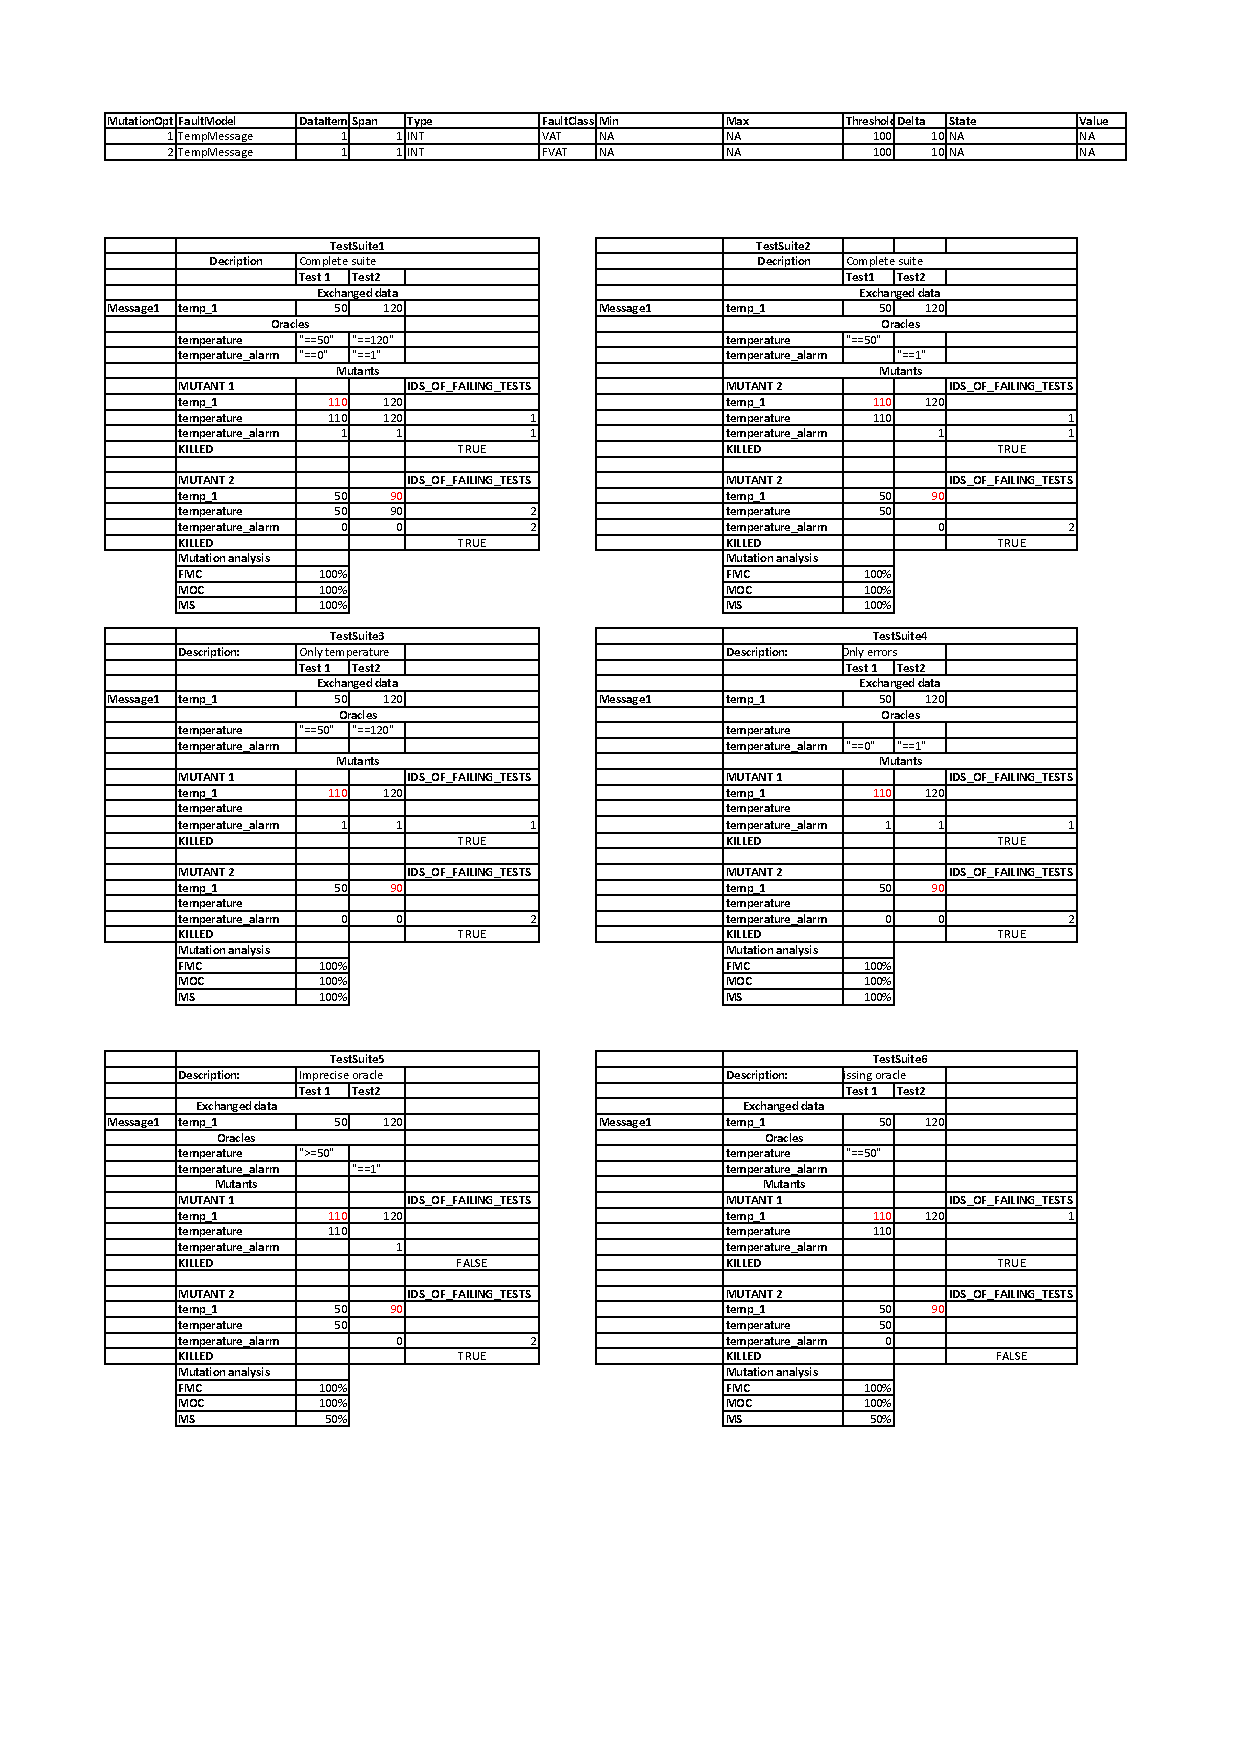
\includegraphics[width=18cm]{damat/DataDrivenExample1A}
\caption{Running example set 1 - Part A.}
\label{fig:damat:RunningExample1A}
\end{figure}

\begin{figure}[tb]
\centering
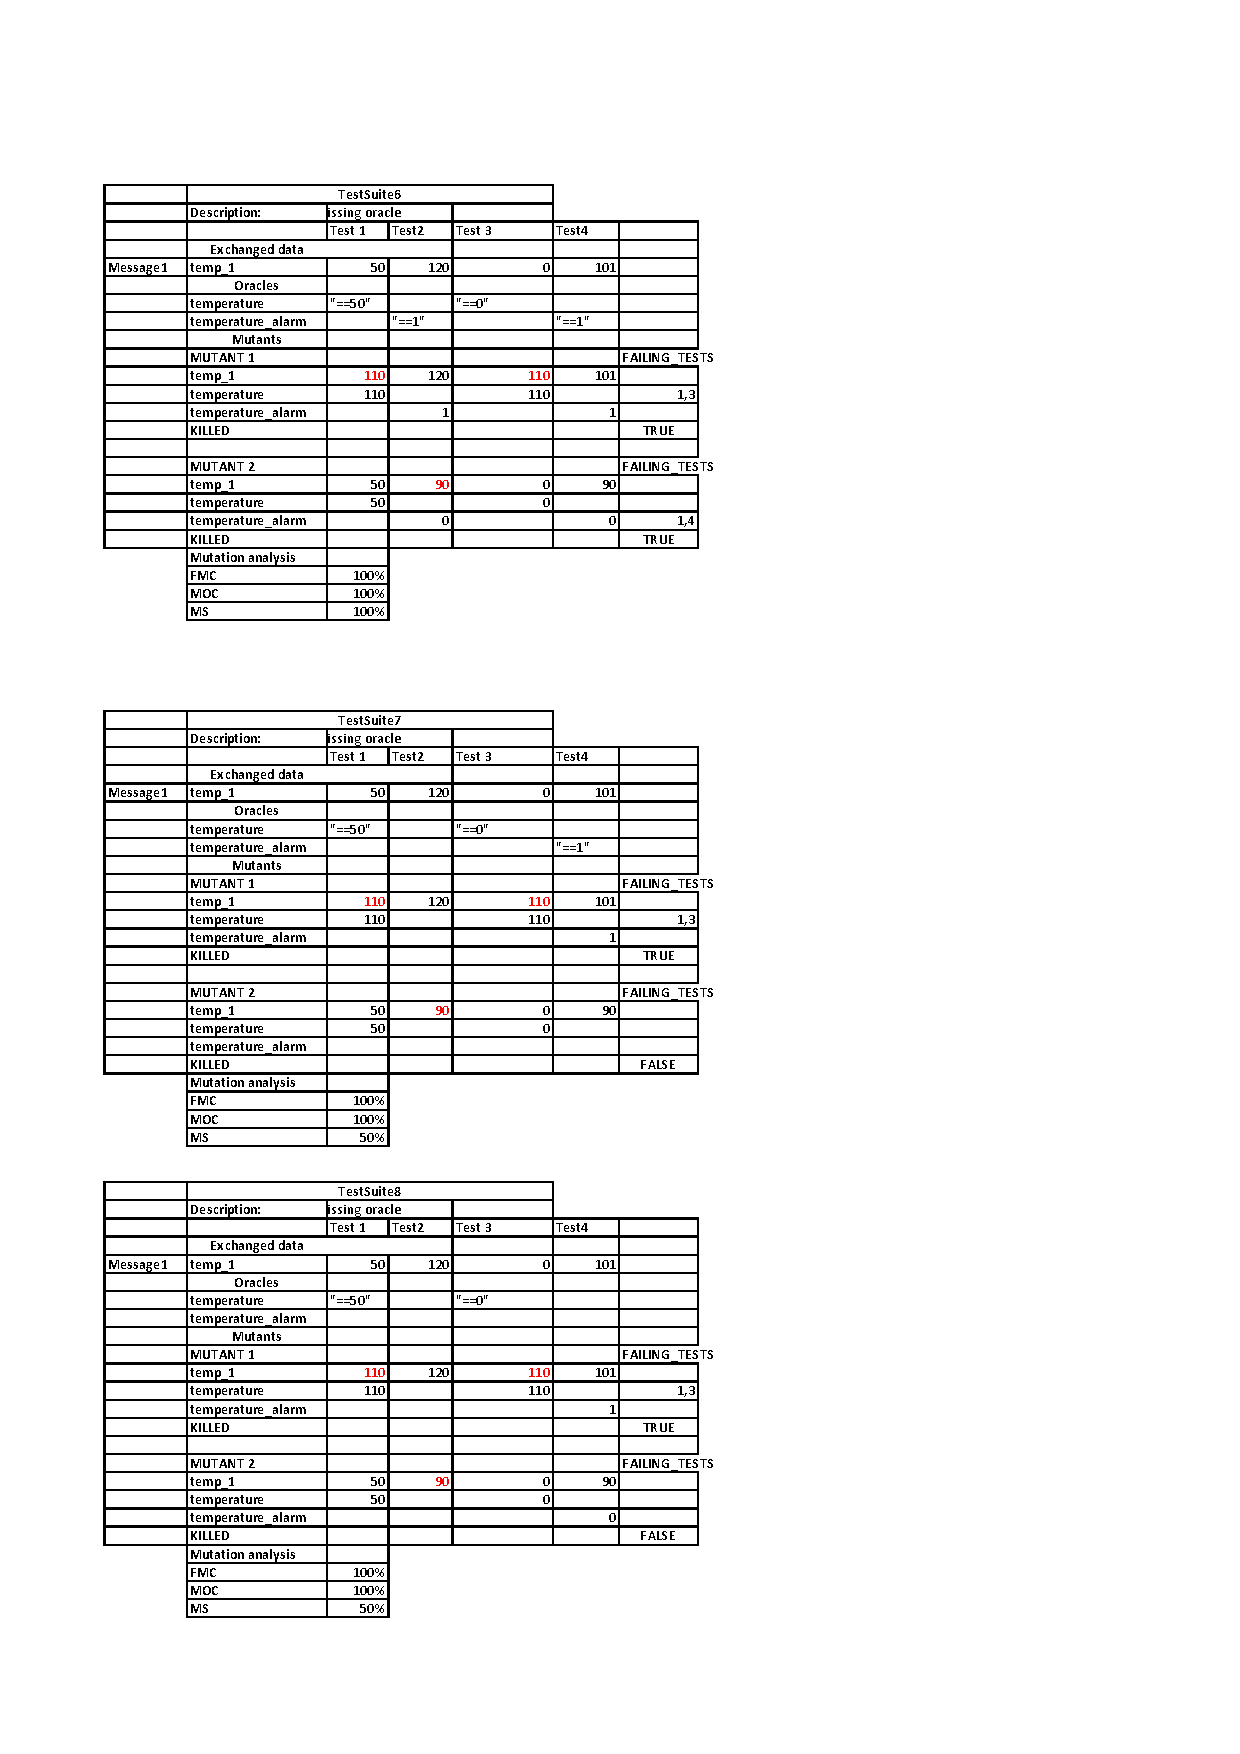
\includegraphics[width=18cm]{damat/DataDrivenExample1B}
\caption{Running example set 1 - Part B.}
\label{fig:damat:RunningExample1B}
\end{figure}

\begin{figure}[tb]
\centering
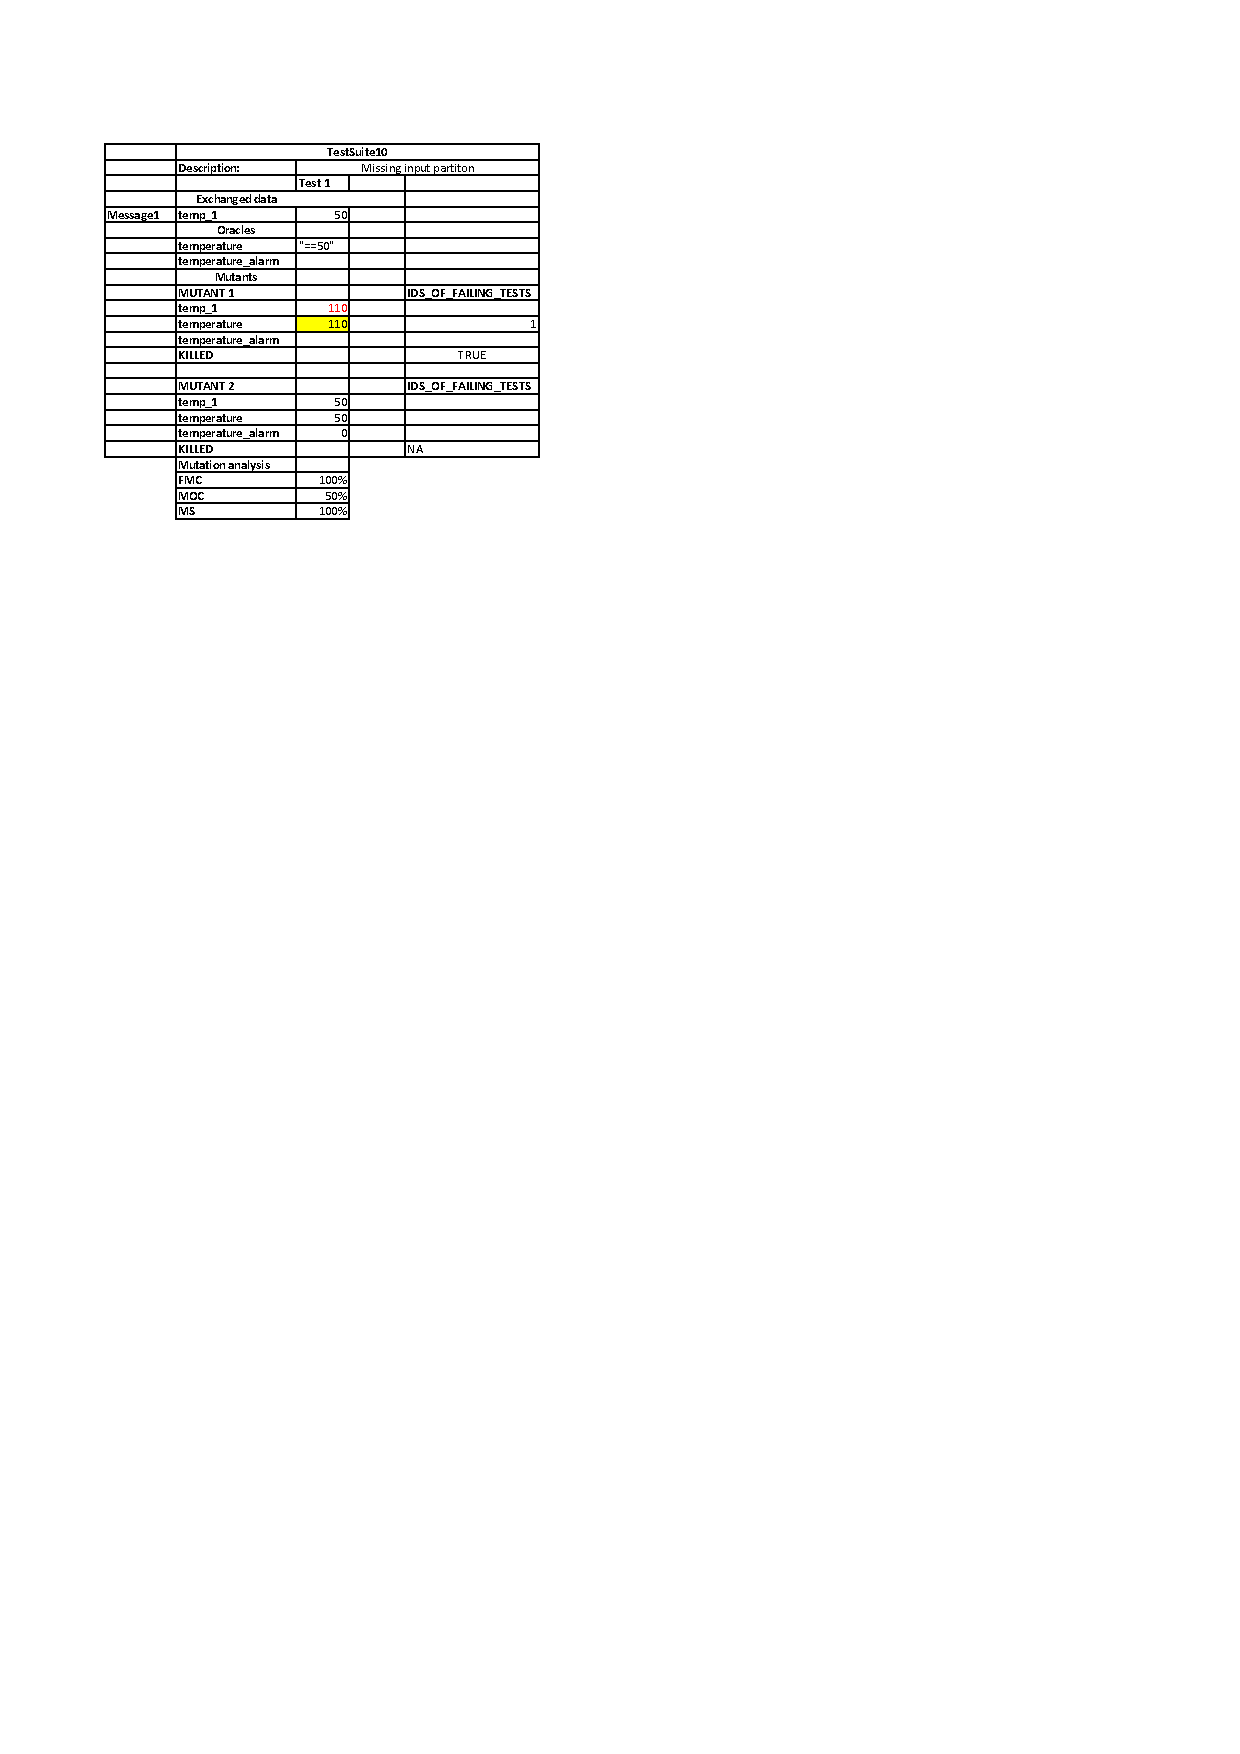
\includegraphics[width=18cm]{damat/DataDrivenExample1C}
\caption{Running example set 1 - Part C.}
\label{fig:damat:RunningExample1C}
\end{figure}

%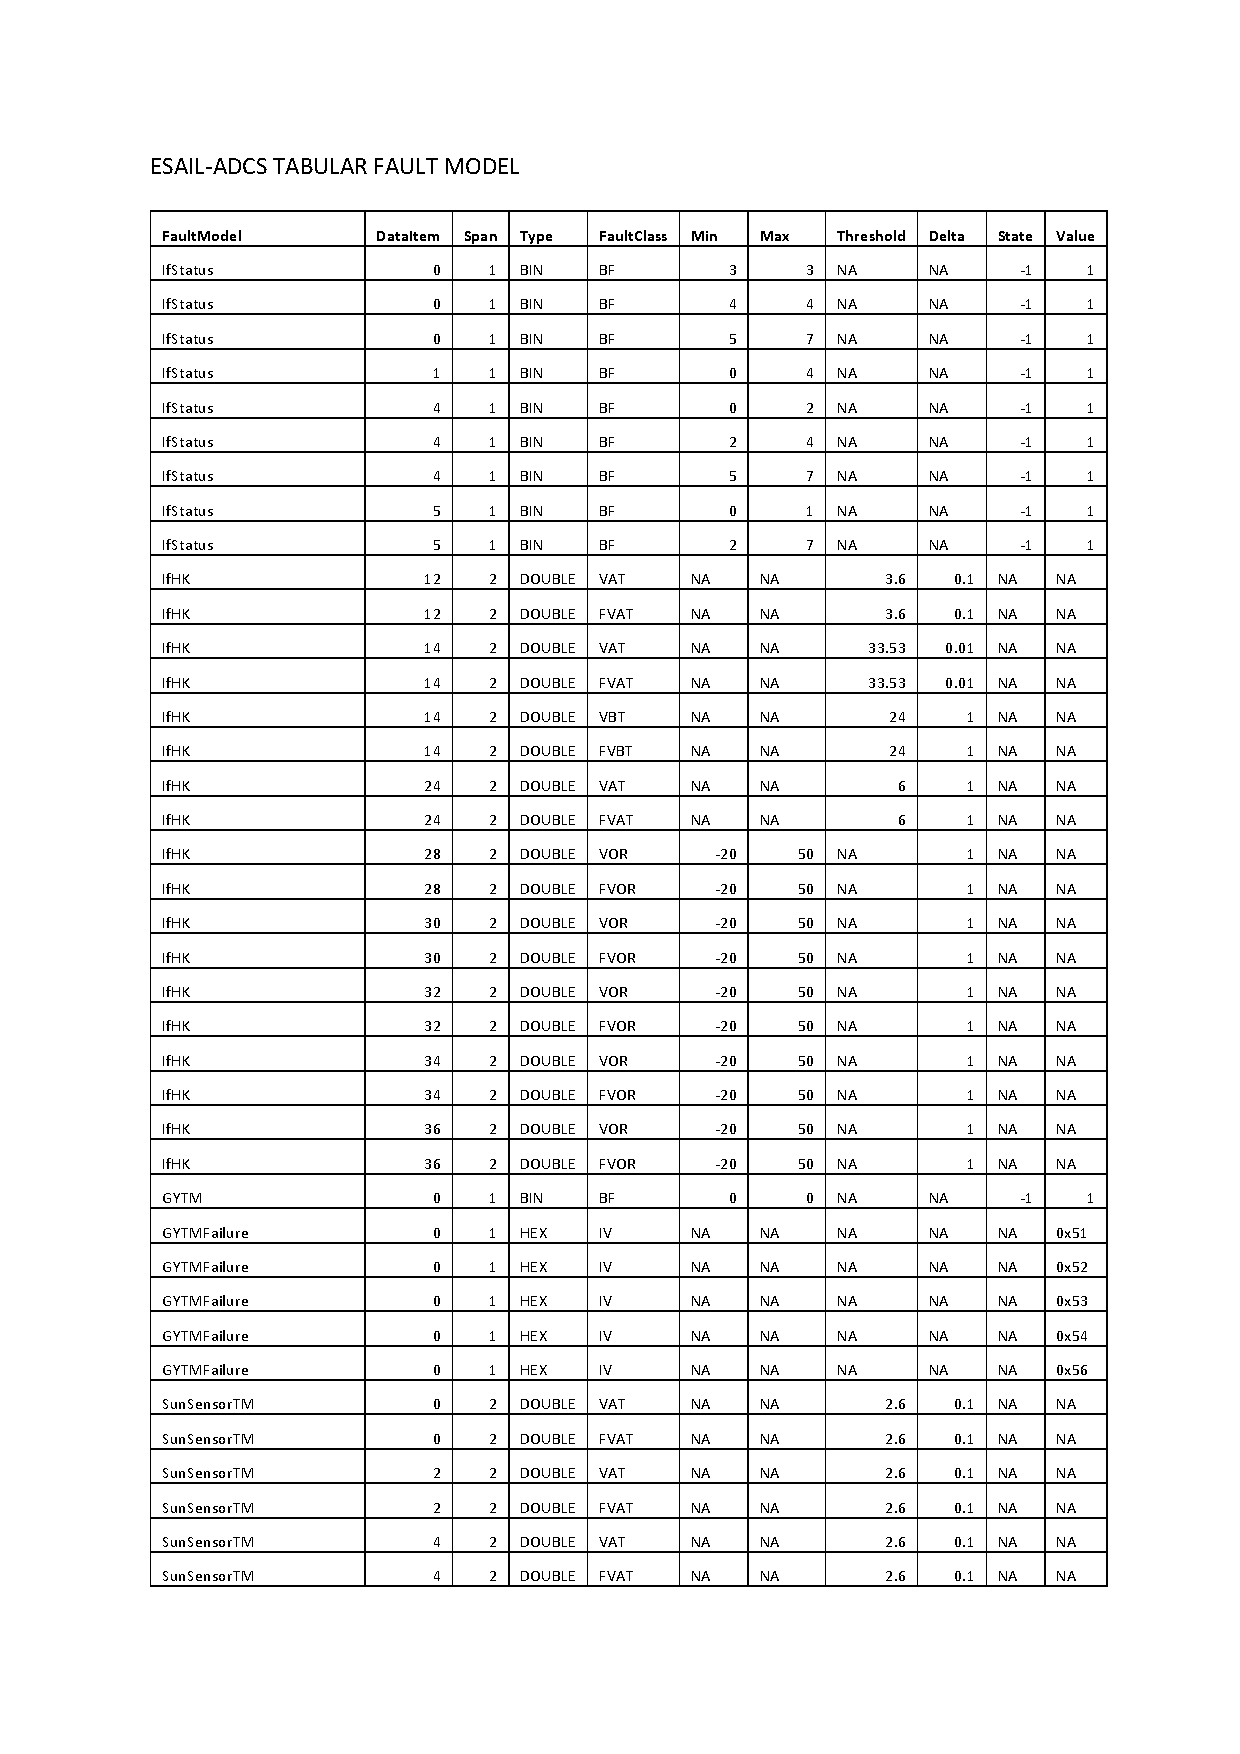
\includepdf[pages=-,scale=0.9,offset=0mm -75]{faultModels/FaultModels.pdf}

\clearpage

\subsubsection{Example set 2: One message exchange, distinct input partitions, faulty software}
\label{sec:dataDriven:example:2}

This running example (see Figure~\ref{fig:damat:RunningExample2}) covers the same case of Section~\ref{sec:dataDriven:example:1}, with the difference that we assume the software to be faulty. More precisely, we assume that the value of \emph{temperature alarm} is always set to 0. We ignore the test suites number 1, 2, 4, 5, 6, 7 because they would detect the presence of the fault before mutation analysis (i.e., the oracles "==1" would fail).

For TestSuite6 and TestSuite8, which do not detect the fault because they lack an oracle for the faulty variable, \APPR would indicate that MUTANT 2 is not killed thus enabling the engineer to introduce an appropriate oracle (i.e., "temperature\_alarm == 1") and thus discover the fault. 

For TestSuite3, \APPR would not help the engineer in detecting the fault because the test suite kills the mutant. What we observe in this case is a sort of masking effect due to the fact that two outputs are affected by the same data; indeed, \APPR ensures that the effect of data mutation is propagated to at least one software output but it cannot verify that the effects of data mutation are propagated to all the software outputs that depend on the mutated data. 
%In this specific case, we would like to highlight that a correct test case would have verified first the presence of temperature_alarms. 
%For the detection of algorithmic faults, code-driven mutation analysis might be more appropriate.

\begin{figure}[tb]
\centering
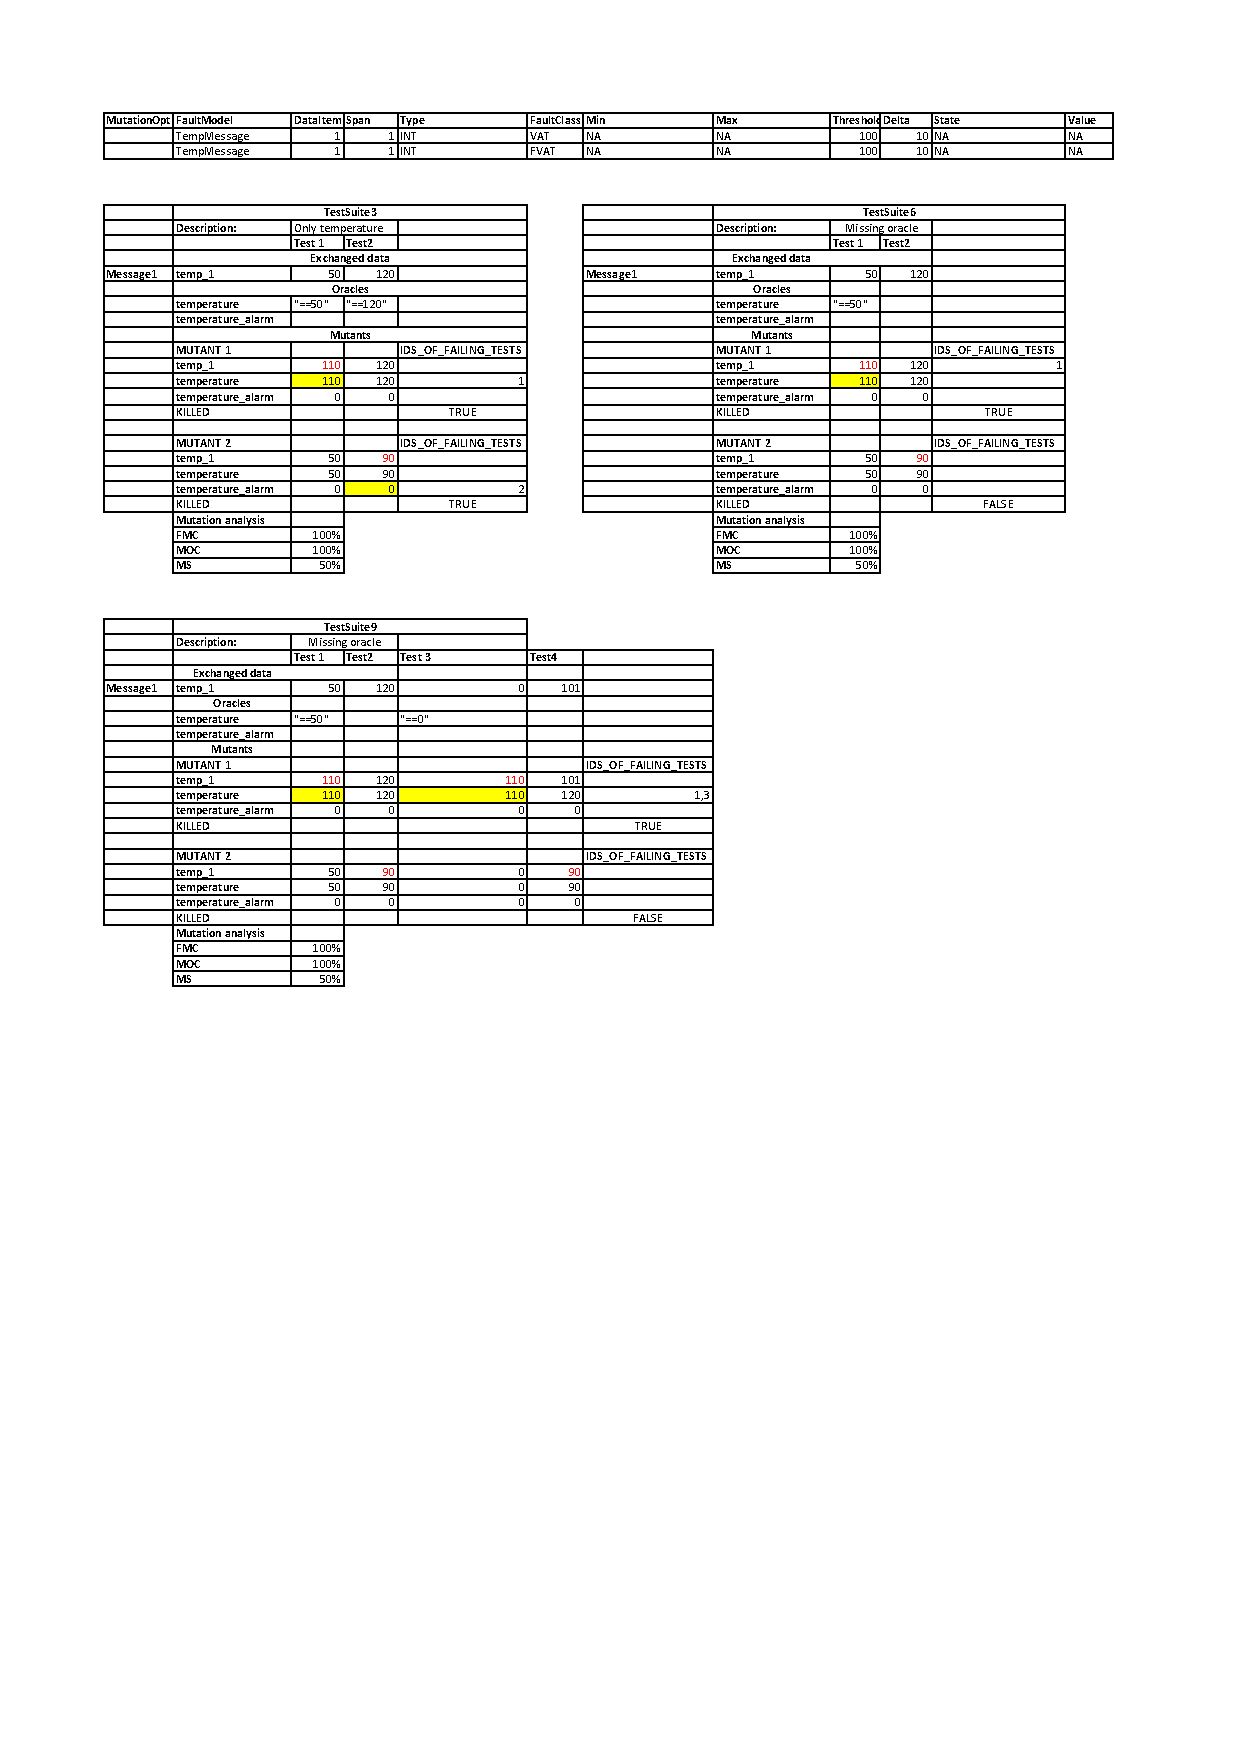
\includegraphics[width=14cm]{damat/DataDrivenExample2}
\caption{Running example set 2.}
\label{fig:damat:RunningExample2}
\end{figure}

\clearpage 
\subsubsection{Example set 3: Multiple message exchanges, distinct input partitions}
\label{sec:dataDriven:example:3}

For the third running example set, we consider a system that has the same architecture of  Figure~\ref{fig:damat:RunningExampleArch} but exchanges also messages of type \emph{BoardStatus}. We assume that \emph{BoardStatus} messages indicate the voltage of the board and the sensors. The SUT has an additional output state variable called \emph{voltage\_error}. A voltage error occurs when the voltage is out of the range (10;14). In the presence of a voltage error, the software shall not update the value of the \emph{temperature} state variable.

Below we discuss two possible test suites, TestSuite1 and TestSuite2, which are affected by different type of limitations.
More precisely, we rely on TestSuite1 to (1) show how \APPR spot a test suite shortcoming difficult to determine manually and (2) demonstrate that \APPR may unlikely lead to equivalent mutants (i.e., by showing that if a mutant is not killed it's because relevant assertions are missing). We rely on TestSuite2 to exemplify the case of lack of coverage of a fault model.

\paragraph{TestSuite1}

Figure~\ref{fig:damat:RunningExample3Sequence} shows the interactions exercised by the test cases in the test suite named TestSuite1 for the running example set 3. Each test case, after starting the ADCS simulator and SUT, waits till the ADCS has sent the following sequence of messages: one BoardStatus message, one TempMessage, one BoardStatus message, and one TempMessage. Then it requests and verifies the values of the state variables \emph{temperature}, \emph{temperature\_alarm}, and \emph{voltage\_error}.

\begin{figure}[tb]
\centering
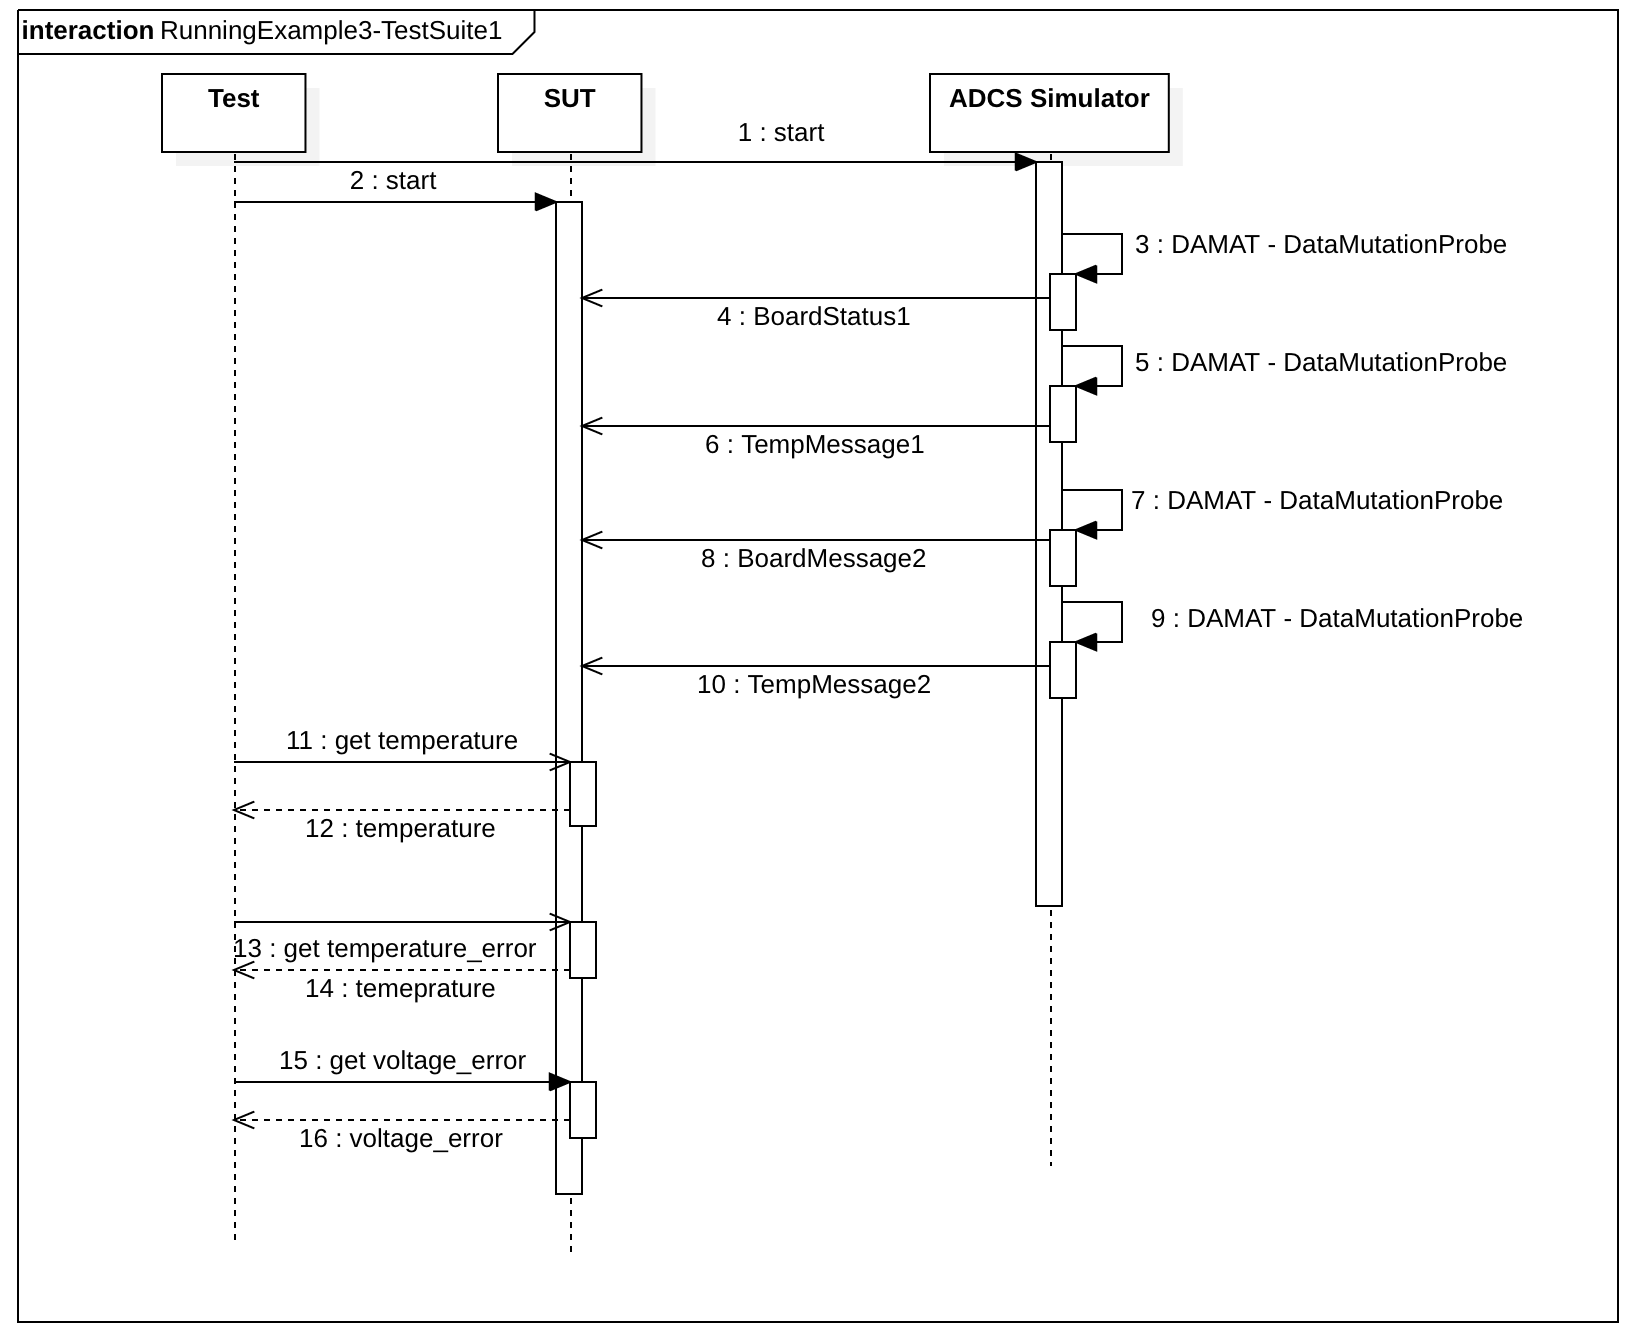
\includegraphics[width=8cm]{damat/images/RunningExampleSequence3.png}
\caption{Interactions exercised by the test cases of TestSuite1 in the running example set 3.}
\label{fig:damat:RunningExample3Sequence}
\end{figure}

Figures~\ref{fig:damat:RunningExample3A} and~\ref{fig:damat:RunningExample3B} show the data exchanged in our running example. With respect to the example set 1, the fault model includes also one VOR and FVOR operator to mutate the BoardStatus message. In Figures~\ref{fig:damat:RunningExample3A} and~\ref{fig:damat:RunningExample3B}, in the row named \emph{PASS}, we explicitly indicate the result of each test case (i.e., PASS or FAIL).

TestSuite1 covers all the possible combinations of values for the sequence of messages reporting about messages voltage error absent (true or false), temperature alarm absent (true or false), voltage error absent (true or false), temperature alarm absent (true or false); indeed, in total, we have 16 test cases.

TestSuite1 kills MUTANT 1. MUTANT 1 applies VAT, that is, it sets the temperature value above the threshold when it is below the threshold. To not kill MUTANT 1, the test suite should not include any failing oracle. Since the failing oracles include the complete set of oracles that either verify the temperature being in the nominal range or verify the absence of a temperature alarm, we conclude that whenever MUTANT 1 is not killed, we cannot be in the presence of an equivalent mutant but in the presence of a test suite limitation.

TestSuite1 kills MUTANT 2. MUTANT 2 applies FVAT, that is, it sets the temperature value below the threshold when it is above the threshold. To not kill MUTANT 2, the test suite shall not include any of the failing oracles. Since the failing oracles include the complete set of oracles that either verify the temperature being out of the nominal range or verify the presence of a temperature alarm, we conclude that whenever MUTANT 2 is not killed, we cannot be in the presence of an equivalent mutant but in the presence of a test suite limitation.

TestSuite1 kills MUTANT 3. MUTANT 3 applies the first mutation procedure of VOR, that is, it sets the value above range if it is within range. To not kill MUTANT 2, the test suite shall not include any of the failing oracles. Since the failing oracles include the complete set of oracles that either verify the temperature being in the nominal range or verify the absence of a temperature alarm, we conclude that whenever MUTANT 3 is not killed, we cannot be in the presence of an equivalent mutant but in the presence of a test suite limitation.

TestSuite1 kills MUTANT 4. MUTANT 4 applies the second mutation procedure of VOR, that is, it sets the value below range if it is in range. MUTANT 4 leads to the same system outputs as MUTANT 3 thus we can make the same conclusion (no equivalent mutant possible).

TestSuite1 kills MUTANT 5. MUTANT 5 applies the first mutation procedure of FVOR, that is, it sets the value within range if it is above range. 
To not kill MUTANT 5, the test suite shall not include any of the failing oracles. All the failing oracles belong to test cases that verify a scenario in which a voltage error is present just before the last temperature message is collected; consequently, the lack of such oracles would indicate a major limitation of the test suites (i.e., it would not test if the software identifies the error condition simulated by the scenario under test). Similarly, MUTANT 5 is killed if all such test cases would be missing; even in this case we would be in the presence of a major test suite limitation (i.e., the test suite does not simulate an important error condition). We thus conclude that MUTANT 5 cannot lead to equivalent mutants. 

TestSuite1 does not kill MUTANT 6. MUTANT 6 applies the second mutation procedure of FVOR, that is, it sets the value in range if it is below range. Since no values below range are observed during the execution of the test cases, \APPR never applies this mutation operation. For this reason the mutation operation for the test suite is 83\% (i.e., five out of six mutation operation are covered). Although TestSuite1 seems complete because it tests all the pairwise combinations of the conditions \emph{voltage error absent} and \emph{temperature alarm absent}, \APPR enables us to determine that when defining the test suite we did not consider the fact that the input partitions for voltage error are three (i.e., voltage within range, voltage above range, and voltage below range) not two (i.e., voltage error absent, voltage error present).




\begin{figure}[tb]
\centering
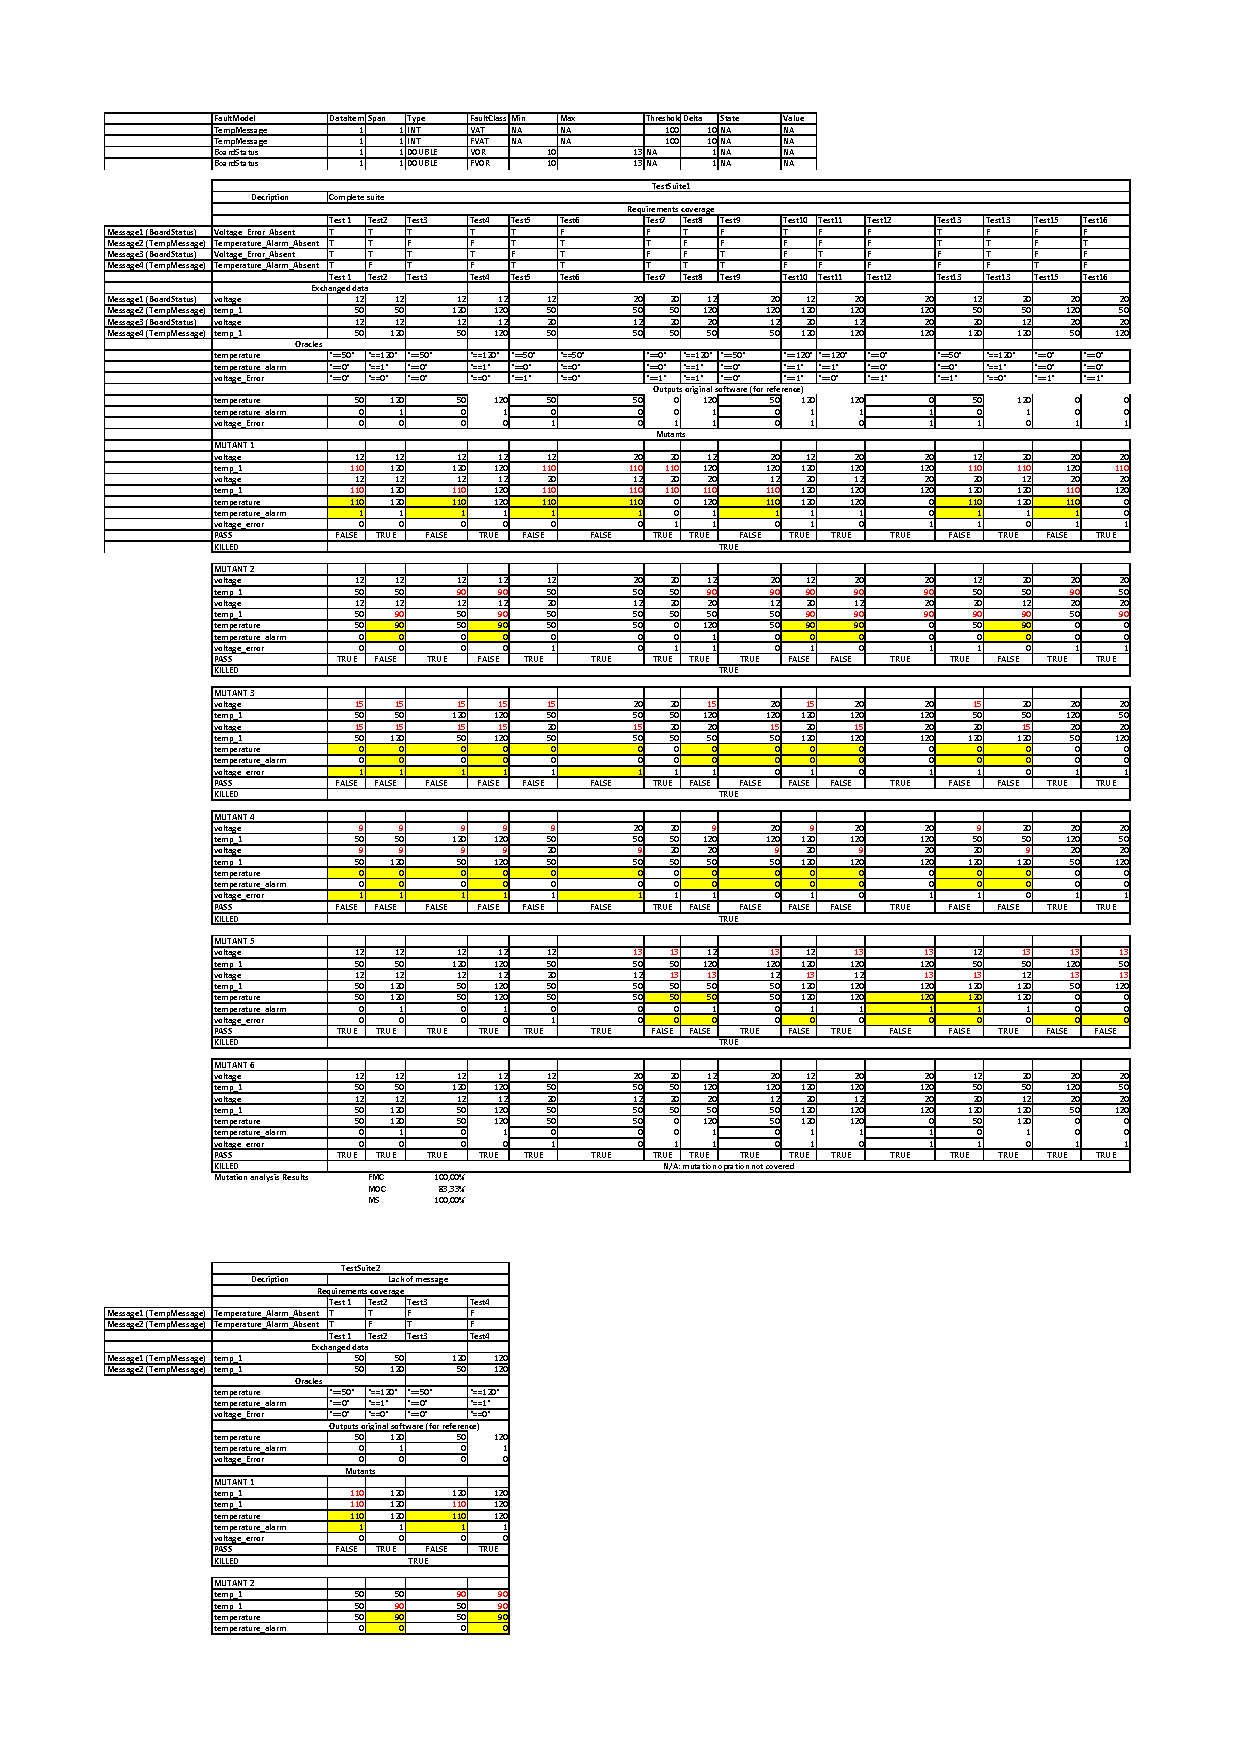
\includegraphics[width=18cm]{damat/DataDrivenExample3A}
\caption{Running example set 3 - Part A.}
\label{fig:damat:RunningExample3A}
\end{figure}

\begin{figure}[tb]
\centering
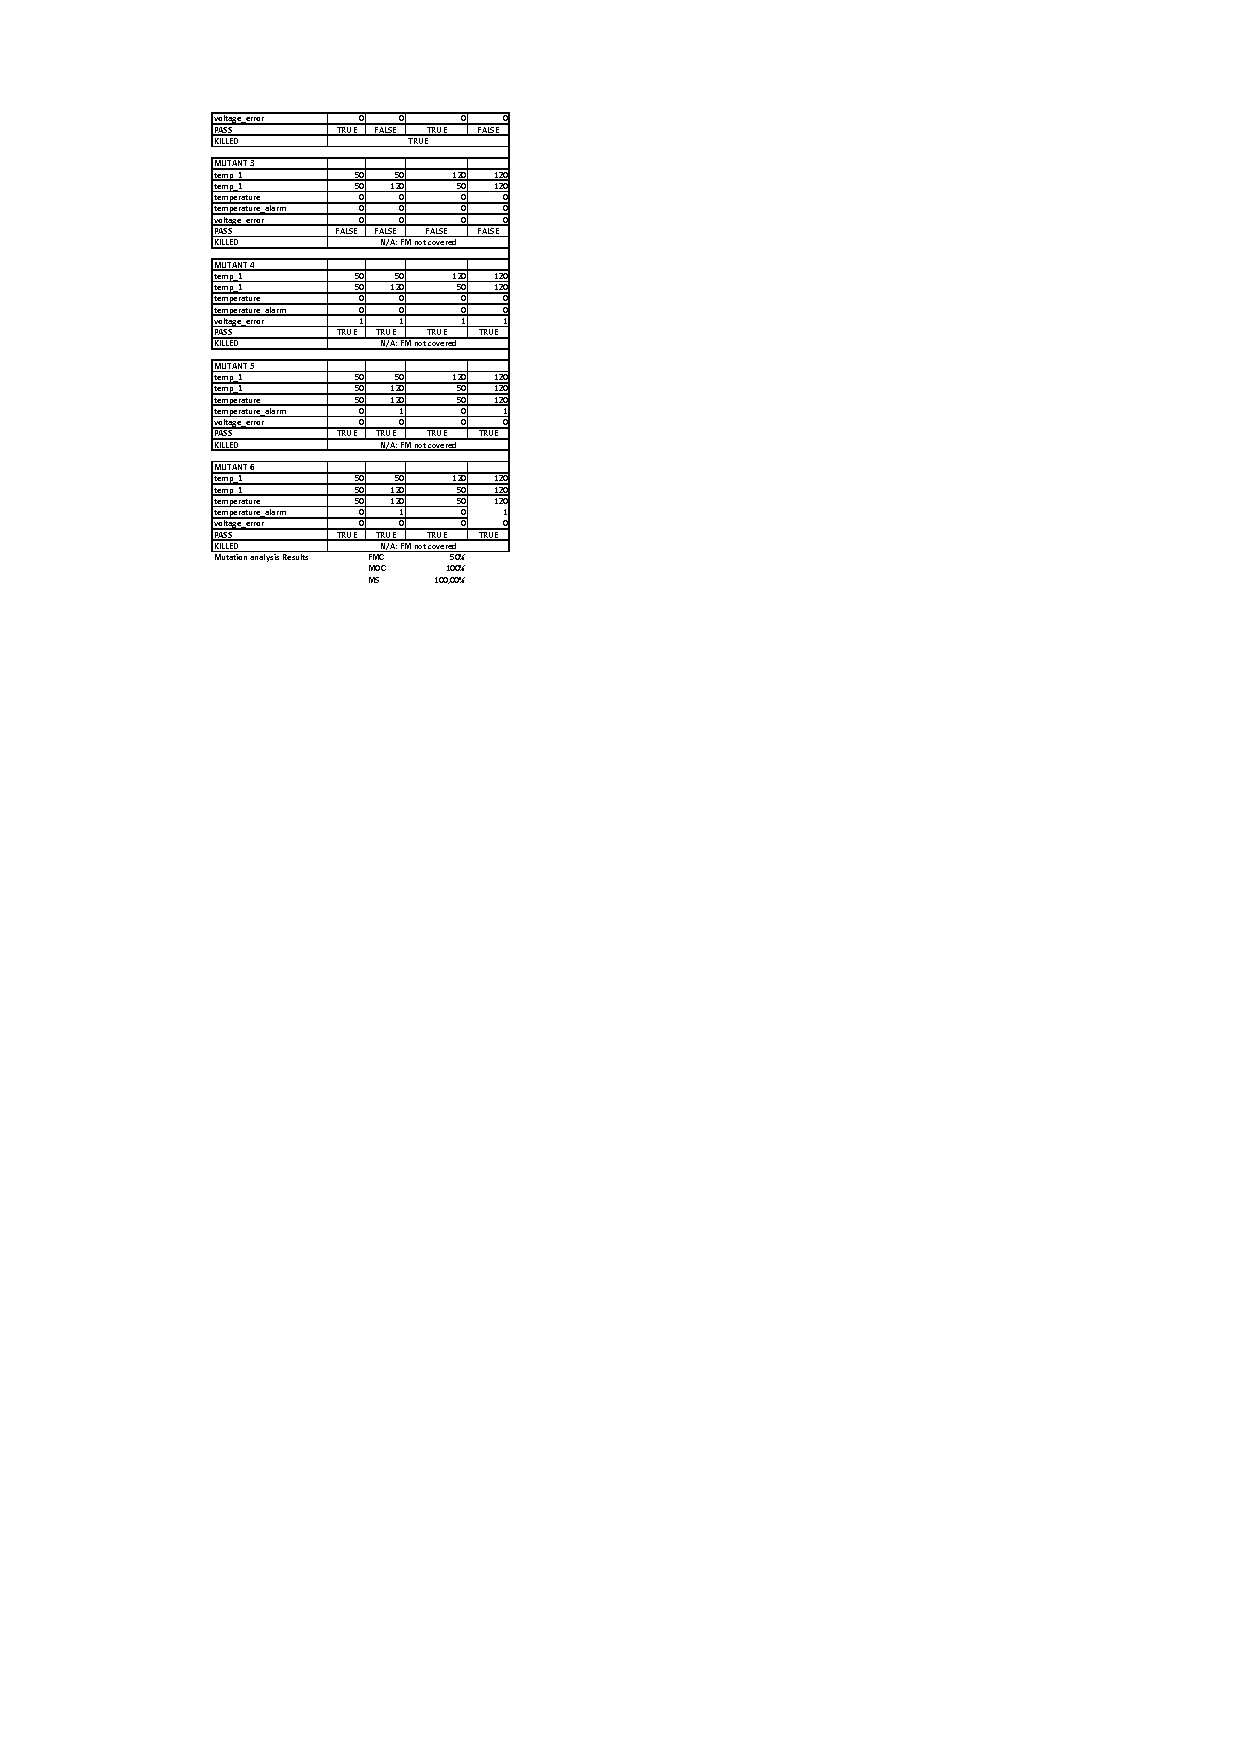
\includegraphics[width=18cm]{damat/DataDrivenExample3B}
\caption{Running example set 3 - Part B.}
\label{fig:damat:RunningExample3B}
\end{figure}


\paragraph{TestSuite2}



\begin{figure}[tb]
\centering
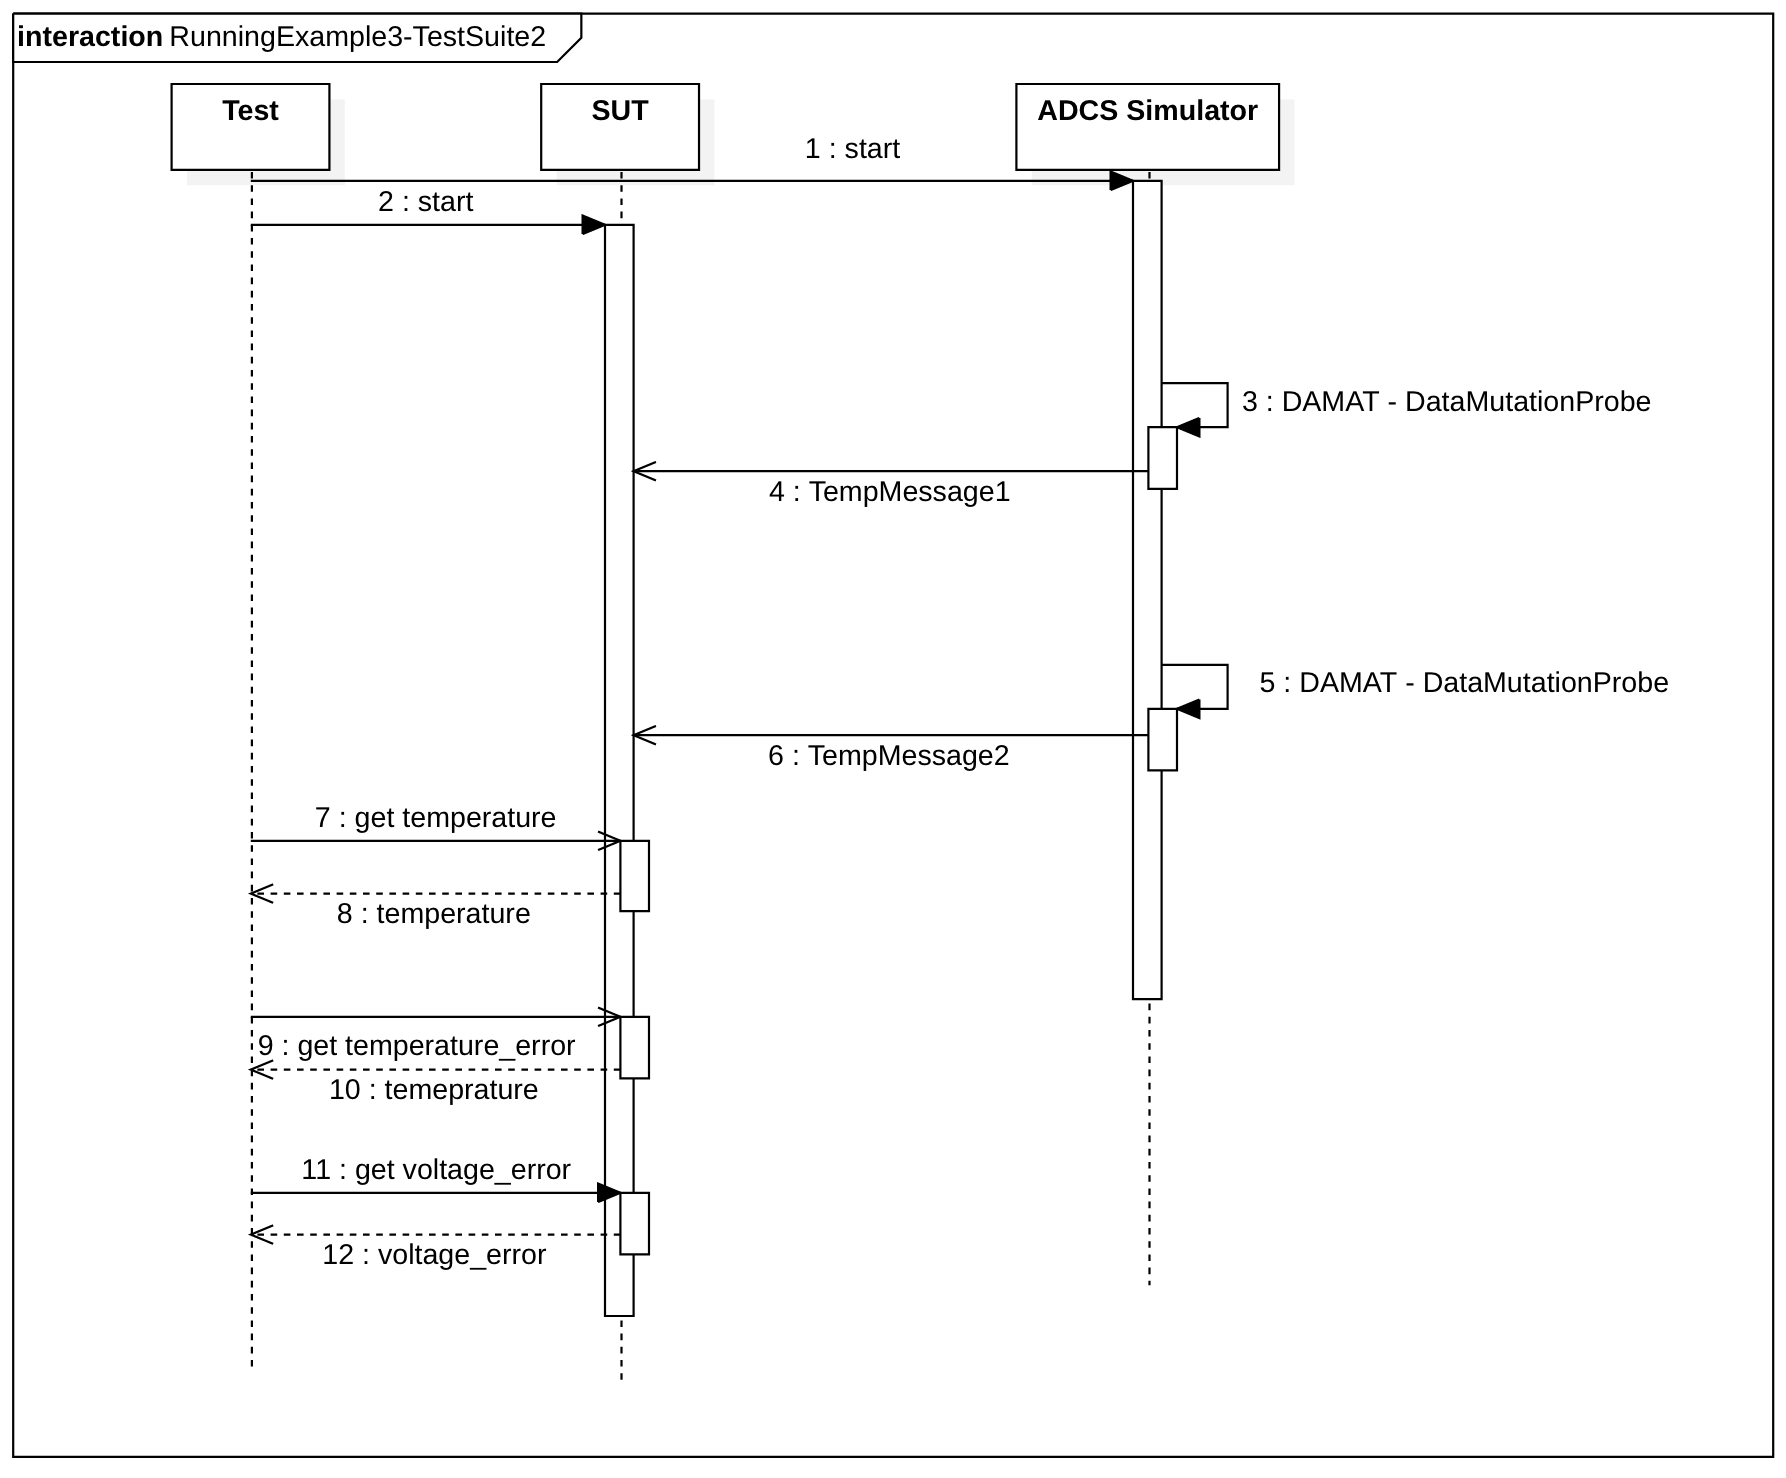
\includegraphics[width=8cm]{damat/images/runningExamplesSequence3_2.png}
\caption{Interactions exercised by the test cases of TestSuite2 in the running example set 3.}
\label{fig:damat:RunningExample3Sequence2}
\end{figure}

TestSuite 2 does not trigger messages of type BoardStatus; its interactions are depicted in Figure~\ref{fig:damat:RunningExample3Sequence2}. For the remaining message type (i.e., TempMessage) it covers all the possible combinations of temperature alarms being present/absent for two TempMessages sent in sequence; in total, we have 4 test cases.

The fault model BoardStatus is not covered; therefore the fault model coverage (FMC) is 50\%. Since MUTANTS 3 to 6 belong to BoardStatus they are not considered in the computation of the other mutation analysis metrics. MOC and MS are thus 100\%; indeed all the mutants not belonging to BoardStatus are killed by the test suite.

MUTANT 1 could be live only if relevant oracles are missing; more precisely, only if oracles concerning the nominal temperature value are missing. MUTANT 1 is killed by TestSuite2.

MUTANT 2 could be live only if relevant oracles are missing; indeed, only if oracles concerning the non nominal temperature value are missing. MUTANT 2 is killed by TestSuite2.